%%%%%%%%%%%%%%%%%%%%%%%%%%%%%%%%%%%%%%%%%%%%%%%%%%%%%%%%%%%%%%%%%%%%%%%%%%%%%%%%
%2345678901234567890123456789012345678901234567890123456789012345678901234567890
%        1         2         3         4         5         6         7         8
\documentclass[letterpaper, 10 pt, conference]{ieeeconf}  % Comment this line out if you need a4paper
% fix acrobat png issue bug
\pdfminorversion=4
%\documentclass[a4paper, 10pt, conference]{ieeeconf}      % Use this line for a4 paper

\IEEEoverridecommandlockouts                              % This command is only needed if 
                                                          % you want to use the \thanks command

\overrideIEEEmargins                                      % Needed to meet printer requirements.

% See the \addtolength command later in the file to balance the column lengths
% on the last page of the document

% The following packages can be found on http:\\www.ctan.org
%\usepackage{graphics} % for pdf, bitmapped graphics files
%\usepackage{epsfig} % for postscript graphics files
%\usepackage{mathptmx} % assumes new font selection scheme installed
%\usepackage{times} % assumes new font selection scheme installed
%\usepackage{amsmath} % assumes amsmath package installed
%\usepackage{amssymb}  % assumes amsmath package installed

\usepackage{balance}
%\usepackage{subfigure}
%\usepackage[subfigure]{tocloft} 


%\usepackage[colorlinks]{hyperref}
%\usepackage[caption=false]{subfig}


\usepackage{caption}
%\usepackage{subcaption}
\captionsetup{compatibility=false}
\captionsetup{font={footnotesize}}


\usepackage{subcaption}
\usepackage{benktools}
\usepackage{tikz}
\usetikzlibrary{external}
\usetikzlibrary{positioning,shapes,shadows,arrows, calc, fit, backgrounds, arrows, positioning}
\tikzexternalize[prefix=tikz/]

\newtheorem{lemma}{Lemma}
\newtheorem{theorem}{Theorem}
\usepackage{amsmath,graphics}
\usepackage{amssymb} 
\usepackage{nicefrac, multirow}
\usepackage{tikz}
\usepackage{bigstrut}
\usepackage{subcaption}

\setlength\bigstrutjot{3pt}
%\usepackage{pgfplots}
%\pgfplotsset{compat=newest}
\usepackage{subfig}
\usepackage{textcomp}
\usetikzlibrary{backgrounds}
\numberwithin{equation}{section} \newtheorem{thm}{Theorem}[section]  
\newtheorem{cor}[thm]{Corollary}    % Corollary environment
\newtheorem{lem}[thm]{Lemma}        % Lemma environment
\newtheorem{dfn}[thm]{Definition}        % Lemma environment
\newtheorem{prop}[thm]{Proposition}  % Proposition environment
\newtheorem{rem}[thm]{Remark}  % Proposition environment
\newtheorem{con}[thm]{Conjecture}  % Proposition environment
\newcommand{\cS}{\mathcal{S}}
\newcommand{\cR}{\mathcal{R}}
\newcommand{\cD}{\mathcal{D}}
\newcommand{\cN}{\mathcal{N}}
\newcommand{\ceq}{\ensuremath{\mathrel{\stackrel{\mathrm{def}}{=}}}} 
\DeclareMathOperator*{\argmin}{arg\,min}
\DeclareMathOperator*{\argmax}{arg\,max}
\newcommand{\rd}{{\mathrm d}}
\newcommand{\p}{\partial}
\tikzstyle{every node}=[font=\small]
%\usepackage{filemod}
\newcommand{\includetikz}[2]{%
\tikzsetnextfilename{#2}%
    \filemodCmp{#1#2.tikz}{#1tikz/#2.pdf}%
        {\tikzset{external/remake next}}{}%
    \input{#1#2.tikz}%
}

\DeclareMathOperator{\J}{J} 
\DeclareMathOperator{\clamp}{clamp} 
\DeclareMathOperator{\interior}{int} 
\DeclareMathOperator{\D}{D} 
\DeclareMathOperator{\Div}{div} 
\DeclareMathOperator{\Sgn}{Sgn} 
\DeclareMathOperator{\Hom}{Hom} 
\DeclareMathOperator{\rank}{rank} 
\DeclareMathOperator{\Vol}{Vol}
\DeclareMathOperator{\Area}{Area}
\DeclareMathOperator{\dVol}{dVol}
\DeclareMathOperator{\supp}{supp} 
\DeclareMathOperator{\Int}{Int} 
\DeclareMathOperator{\Conv}{Conv} 
\DeclareMathOperator{\Cone}{Cone} 
\DeclareMathOperator{\Ker}{Ker} 
\DeclareMathOperator{\Span}{Span} 
\DeclareMathOperator{\Min}{Min} 
\newcommand{\bone}{\mathbf{1}}
\DeclareMathOperator{\tr}{tr} 
\newcommand{\bR}{\mathbb{R}} 
\newcommand{\bZ}{\mathbb{Z}}
\newcommand{\bbeta}{\boldsymbol{\beta}}
\newcommand{\balpha}{\boldsymbol{\alpha}}
\newcommand{\bE}{\mathbb{E}}
\newcommand{\bI}{\mathbb{I}}
\newcommand{\bQ}{\mathbb{Q}}
\newcommand{\bK}{\mathbb{K}}
\newcommand{\bL}{\mathbb{L}} 
\newcommand{\bB}{\mathbb{B}} 
\newcommand{\bbT}{\mathbb{T}} 
\newcommand{\bN}{\mathbb{N}}
\newcommand{\cJ}{\mathcal{J}}
\newcommand{\cI}{\mathcal{I}}
\newcommand{\bS}{\mathbb{S}}
\newcommand{\cL}{\mathcal{L}}
\newcommand{\cF}{\mathcal{F}}
\newcommand{\cH}{\mathcal{H}}
\newcommand{\cU}{\mathcal{U}}
\newcommand{\cK}{\mathcal{K}}
\newcommand{\cB}{\mathcal{B}}
\newcommand{\cV}{\mathcal{V}}
\newcommand{\cZ}{\mathcal{Z}}
\newcommand{\cW}{\mathcal{W}}
\newcommand{\cO}{\mathcal{O}} 
\newcommand{\cC}{\mathcal{C}}
\newcommand{\cT}{\mathcal{T}}
\newcommand{\bbF}{\mathbb{F}}
\newcommand{\cA}{\mathcal{A}}
\newcommand{\cM}{\mathcal{M}}
\newcommand{\cG}{\mathcal{G}}
\newcommand{\cKG}{\mathcal{KG}}
\renewcommand{\phi}{\varphi}
\renewcommand{\div}{\mbox{div}}
\newcommand{\ve}{\varepsilon}
\newcommand{\norm}[1]{\lVert #1 \rVert}
\newcommand{\abs}[1]{\left| #1 \right|}
\newcommand{\ov}[1]{\overline{#1}}
\newcommand{\diff}[4]{\left.\left.\frac{\operatorname{d}}{\operatorname{d}#1}\right.^{#2}#3\right|_{#4}}
\renewcommand{\geq}{\geqslant}
\renewcommand{\leq}{\leqslant}
\renewcommand{\ge}{\geqslant}
\renewcommand{\le}{\leqslant}

\newcommand{\furlp}[1]{\colorbox{blue!10}{\href{run:/home/fulong/academia/library/papers/#1.pdf}{D}}}
\newcommand{\furlb}[1]{\colorbox{blue!10}{\href{run:/home/fulong/academia/library/books/#1.pdf}{D}}}
\newcommand{\fcitep}[1]{\cite{#1}\mbox{\furlp{#1}}}
\newcommand{\fciteb}[1]{\cite{#1}\mbox{\furlb{#1}}}
% we can now use cite as before
% misc defines
\newcommand{\bx}{\mathbf{x}}
\newcommand{\hbx}{\hat{\mathbf{x}}}
\newcommand{\bbx}{\bar{\mathbf{x}}}
\newcommand{\sbx}{\mathbf{x}^{\star}}
\newcommand{\ba}{\mathbf{a}}
\newcommand{\bu}{\mathbf{u}}
\newcommand{\bc}{\mathbf{c}}
\newcommand{\bg}{\mathbf{g}}
\newcommand{\by}{\mathbf{y}}
\newcommand{\bz}{\mathbf{z}}
\newcommand{\bbf}{\mathbf{f}}
\newcommand{\bt}{\mathbf{t}}
\newcommand{\bh}{\mathbf{h}}
\newcommand{\bn}{\mathbf{n}}
\newcommand{\bp}{\mathbf{p}}
\newcommand{\bq}{\mathbf{q}}
\newcommand{\bv}{\mathbf{v}}
\newcommand{\br}{\mathbf{r}}
\newcommand{\bs}{\mathbf{s}}
\newcommand{\bb}{\mathbf{b}}
\newcommand{\bC}{\mathbf{C}}
\newcommand{\bF}{\mathbf{F}}
\newcommand{\bP}{\mathbf{P}}
\newcommand{\bT}{\mathbf{T}}
\newcommand{\bV}{\mathbf{V}}
\newcommand{\hbb}{\hat{\mathbf{b}}}
\newcommand{\hbn}{\hat{\mathbf{n}}}
\newcommand{\bbb}{\bar{\mathbf{b}}}
\newcommand{\hbu}{\hat{\mathbf{u}}}
\newcommand{\bbu}{\bar{\mathbf{u}}}
\newcommand{\bw}{\mathbf{w}}
\newcommand{\mG}{\mathcal{G}}
\newcommand{\mA}{\mathcal{A}}
\newcommand{\mH}{\mathcal{H}}
\newcommand{\mL}{\mathcal{L}}
\newcommand{\mN}{\mathcal{N}}
\newcommand{\mE}{\mathcal{E}}
\newcommand{\mO}{\mathcal{O}}
\newcommand{\mP}{\mathcal{P}}
\newcommand{\mB}{\mathcal{B}}
\newcommand{\mC}{\mathcal{C}}
\newcommand{\mX}{\mathcal{X}}
\newcommand{\mY}{\mathcal{Y}}
\newcommand{\mZ}{\mathcal{Z}}
\newcommand{\mW}{\mathcal{W}}
\newcommand{\mQ}{\mathcal{Q}}
\newcommand{\mR}{\mathcal{R}}
\newcommand{\mU}{\mathcal{U}}
\newcommand{\mD}{\mathcal{D}}
\newcommand{\mF}{\mathcal{F}}
\newcommand{\mS}{\mathcal{S}}
\newcommand{\mK}{\mathcal{K}}
\newcommand{\mV}{\mathcal{V}}
\newcommand{\mI}{\mathcal{I}}
\newcommand{\bG}{\mathbf{G}}
\newcommand{\bA}{\mathbf{A}}
\newcommand{\bW}{\mathbf{W}}
\newcommand{\hmX}{\hat{\mathcal{X}}}
\newcommand{\hmU}{\hat{\mathcal{U}}}
\newcommand{\bmX}{\bar{\mathcal{X}}}
\newcommand{\bmU}{\bar{\mathcal{U}}}
\newcommand{\mT}{\mathcal{T}}
\newcommand{\mM}{\mathcal{M}}
\newcommand{\bPhi}{\boldsymbol{\Phi}}
\newcommand{\bGamma}{\boldsymbol{\Gamma}}
\newcommand{\hbpsi}{\hat{\boldsymbol \psi}}
\newcommand{\bPsi}{\boldsymbol \Psi}
\newcommand{\bpsi}{\boldsymbol{\psi}}
\newcommand{\sS}[1]{\sqrt{\Sigma_{#1}}}
\newcommand{\shS}[1]{\sqrt{\hat{\Sigma}_{#1}}}
\newcommand{\sd}{\texttt{sd}}
\DeclareMathOperator{\Cov}{Cov}
\DeclareMathOperator{\Tr}{tr}
\DeclareMathOperator{\st}{s.t.}
\DeclareMathOperator{\dt}{dt}
\DeclareMathOperator{\Vect}{vec}
\DeclareMathOperator{\diag}{diag}
%\DeclareMathOperator{\argmin}{arg\,min}

\captionsetup{font={footnotesize}}

\newcommand{\specialcell}[2][c]{ \begin{tabular}[#1]{@{}c@{}}#2\end{tabular}}

\newcommand\independent{\protect\mathpalette{\protect\independenT}{\perp}}
\def\independenT#1#2{\mathrel{\rlap{$#1#2$}\mkern2mu{#1#2}}}

\newcommand{\limit}[1] {\underset{#1}{\text{lim }}}
\newcommand{\infimum}[1] {\underset{#1}{\text{inf }}}
\newcommand{\supremum}[1] {\underset{#1}{\text{sup }}}
\newcommand{\maximum}[1] {\underset{#1}{\text{max }}}
\newcommand{\minimum}[1] {\underset{#1}{\text{min }}}
\newcommand{\myargmax}[1] {\underset{#1}{\text{argmax }}}
\newcommand{\myargmin}[1] {\underset{#1}{\text{argmin }}}
\newcommand{\betadist}{\text{Beta}}

\newcommand{\TODO}[1]{\todo{#1}}


\begin{document}
\title{\LARGE \bf DexNet 1.0: Correlated Multi-Armed Bandit Models for Large Scale 3D Grasp Planning Under Uncertainty}
\author{Jeffrey Mahler, Brian Hou, Mel Roderick, Michael Laskey, Florian Pokorny, Ken Goldberg}
%\institute{Deptartment of Electrial Engineering and Computer Sciences, University of California, Berkeley, USA
%\{jmahler, zmccarthy, sachinpatil, pabbeel, goldberg\}@berkeley.edu} 
\maketitle

%\begin{abstract}
%\TODO{Adapted from flyer, probably needs to be toned down}
Advances in Big Data and distributed computing, combined with very large datasets of images and human speech, have produced a series of  data-driven results that surpass decades of research in analytic methods and, in some cases, that surpass human ability.
For example, deep neural networks can now learn to play video games, recognize faces, and translate between languages.
This raises the question: can Big Data and computation produce analogous advances in robot grasping and manipulation?
We introduce the Dexterity-Network (Dex-Net) 1.0, a Cloud-based dataset of 3D object models labelled with parallel-jaw grasps and similarity between objects and grasps based on multi-view Convolutional Neural Networks (CNNs) and grasp heightmaps.
We use Dex-Net in Multi-Armed Bandit (MAB) algorithms to quickly find a grasp with high probability of force closure on an object from a set of 250 candidates. 
We extend previous MAB models to predict grasp quality using similiarity to prior objects and grasps in Dex-Net using Continuous Correlated Beta Processes (CCBPs).
Our initial results suggest that using prior objects from Dex-Net can accelerate grasp planning by up to $10\times$.
%\TODO{More concrete results here as I organize them} 
Code, data, and additional information can be found at: \TODO{Url}
\end{abstract}
%
\section{Introduction}
\seclabel{extended-abstract}

Robots in warehouse order fullfillment and small- to medium-scale manufacturing must be able to efficiently grasp and manipulate new products and parts.
For example, a robot processing orders in a distribution warehouse must quickly plan graps for new consumer products to place them in shipping containers. 
% Above motivates speed and adaptivity
% Statement motivating robustness to uncertainty
Furthermore, a robot may not fully observe the state of the workspace, such as the pose or frictional properties of consumer products, due to sensor imprecision and missing data resulting from occlusions.
This poses a challenge for grasp planning with either analytic methods~\cite{ferrari1992, ciocarlie2009} that require precise knowledge of contact locations and surface normals or data-driven approaches~\cite{bohg2014data} that attempt to build a statistical model of grasp success over the massive number of configurations of the environment.
%This motivates an approach to grasp planning that is fast, robust to uncertainty about the state of the robot and environment, and can adapt to new objects and perturbations in the envrionment.

Past work has attempted to overcome this by planning grasps analytically with high probability of force closure~\cite{kehoe2012toward, kim2012physically, laskey2015bandits, mahler2015gp, weisz2012pose}, or using data-driven methods to predict grasp success from human labels~\cite{balasubramanian2012physical, detry2013learning,  herzog2014learning, kappler2015leveraging, lenz2015deep, saxena2008robotic} or empirical successes on a physical robot~\cite{boularias2014efficient, brook2011collaborative, detry2011learning, kroemer2010combining, montesano2012active}.
Many works on grasp selection with probablity of force closure evaluate a set of candidate grasps using sampling and select the highest quality grasp either using brute force sampling~\cite{kehoe2012toward, kim2012physically, weisz2012pose}, iterative pruning~\cite{kehoe2012estimating}, or Multi-Armed Bandit (MAB) algorithms to adaptively sample more promising grasps~\cite{barto1998reinforcement,
lai1985asymptotically, laskey2015bandits, robbins1985some}.
However, MAB algorithms, the current fastest sampling method, still required approximately 10 samples per grasp to converge to a solution and needed to be re-run for every new object.

On the other hand, data-driven approaches have shown promise over analytic methods on physical robot trials~\cite{balasubramanian2012physical, herzog2014learning} possibly due to a reduction in modelling error.
The number of objects and grasps tested is typically on the order of tens to hundreds for physical robot trials and at most a few thousand objects and hundreds of thousands of grasps when using simulation or human labels~\cite{goldfeder2009columbia, lenz2015deep, kappler2015leveraging}.
In comparison, state-of-the-art learning results in image classification~\cite{deng2009imagenet, krizhevsky2012imagenet} and speech recognition~\cite{cieri2004fisher, hannun2014deepspeech} relied on datasets containing tens of millions of examples.
This raises the question: will maching learning for grasp planning under vast numbers of possible object poses, object shapes, environment configurations, etc., exhibit scaling effects similar to those observed in computer vision and speech recognition?
%may require orders of magnitude more data than in use currently.

%This motivated gradient-based methods based on approximations to the probabliity of force closure~\cite{mahler2015gp} and using Multi-Armed Bandit algorithms to adaptively sample more promising grasps~\cite{laskey2015bandits}, which reduced the number of samples until convregence by 10$\times$.
%However, the number of iterations was still prohibitively high for real-time execution and prior knowledge could not be utilized for new objects.

To make progress toward answering this question, we introduce the Dexterity Network (DexNet) 1.0, a dataset of tens of thousands of 3D mesh models and a system for building statistical models that predict grasp quality across the dataset.
DexNet is composed of laser-scanned 3D mesh models from the KIT object database~\cite{kasper2012kit}, the Amazon Picking Challenge objects, BigBIRD~\cite{singh2014bigbird}, and YCB ~\cite{calli2015benchmarking}, and synthetic 3D mesh models from 3DNet~\cite{wohlkinger20123dnet} and the SHREC 2014 large scale object retrieval challenge~\cite{li2015comparison}.
~\figref{dexnet-teaser} shows a subset of the objects in the dataset.
To measure similarity between objects, we form an object network based on Deep Convolutional Neural Networks (CNNs) trained to predict object categories from synthetic rendered images of each object~\cite{aubry2015understanding, li2015comparison}.
The DexNet system uses Google Compute Engine to launch up to 600 instances at a time for evaluating grasp quality on subsets of objects and takes approximately 9.5 hours to run 1,800 objects on 180 instances.

\begin{figure}[t!]
\centering
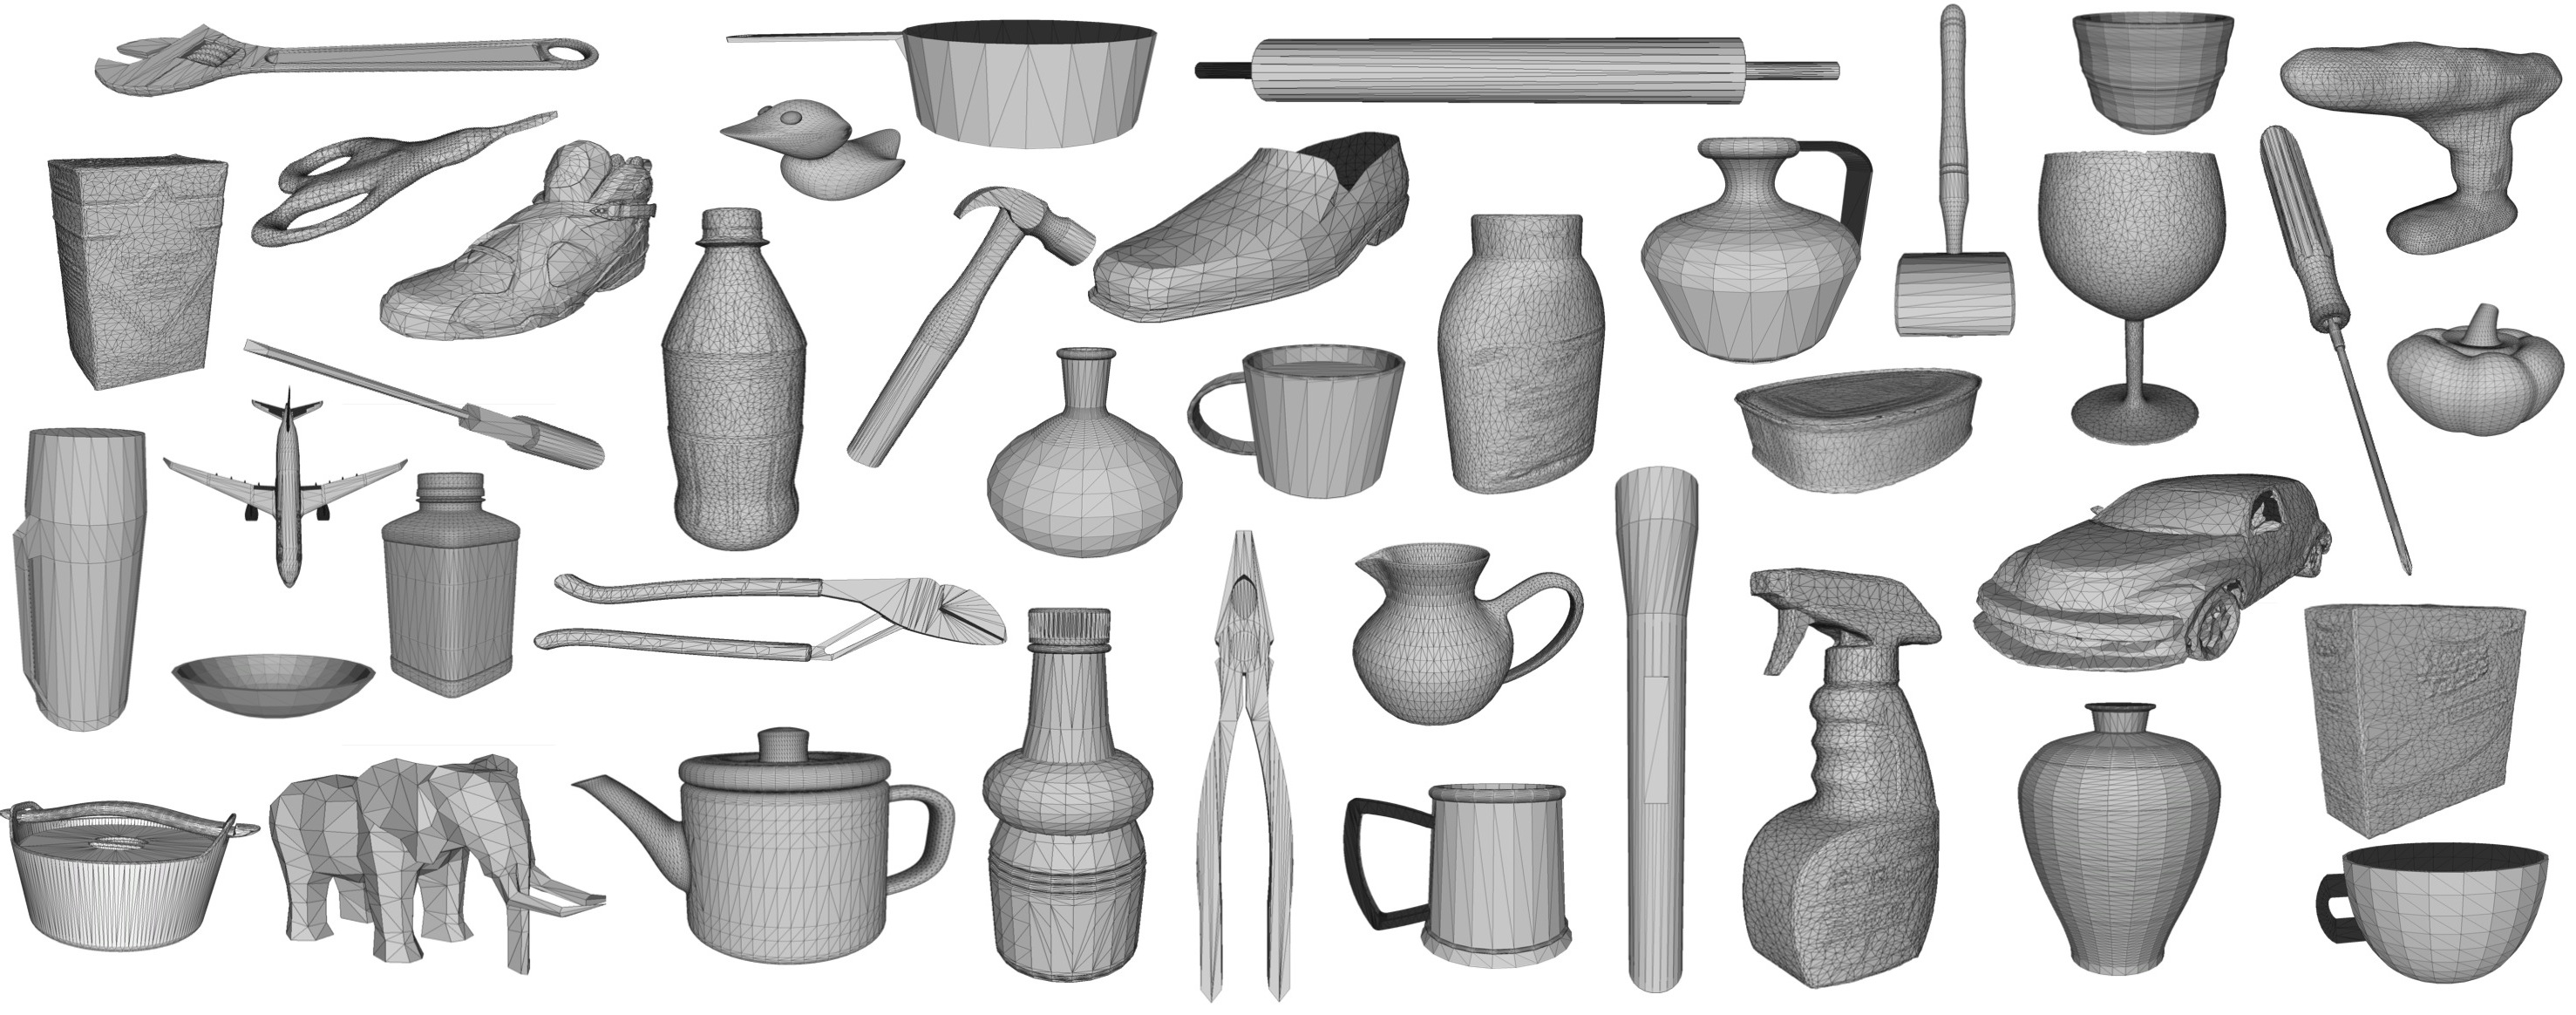
\includegraphics[scale=0.085]{figures/dexnet_collage.jpg}
\caption{Sample of 3D mesh models from the DexNet dataset. The dataset consists of over 30,000 models from laser-scanned datsets such as the KIT object database~\cite{kasper2012kit} and the Yale-CMU-Berkeley object set~\cite{calli2015benchmarking}, and synthetic datasets such as 3DNet\cite{wohlkinger20123dnet} and the SHREC 2014 object retrieval challenge dataset~\cite{li2015comparison} }
\figlabel{dexnet-teaser}
\vspace*{-15pt}
\end{figure}

In this work, we use DexNet to study the number of samples that MAB algorithms take to converge to a grasp with high probability of force closure across orders of magnitude of prior data of grasps with known quality.
To do so, we extend the MAB framework of Laskey et al.~\cite{laskey2015bandits} to model correlations between the probability of force closure for grasps on similar objects using Continuous Correlated Beta Processes (CCBPs)~\cite{goetschalckx2011continuous, montesano2012active}.
CCBPs allow us to form a prior belief on the quality of candidate grasps for a new object based on data in DexNet and to efficiently update a global belief on the quality of all candidate grasps on an object after observing the outcome of a single sampled grasp.
We measure local similarities between grasps on the same object by a distance between the gripper poses and the similarity between local surface patches near the mean location of contact on the object~\cite{herzog2014learning, kappler2015leveraging}.
We measure global similarity in shape based on the distance between the objects in DexNet.
While we acknowledge probability of force closure has shortcomings~\cite{balasubramanian2012physical}, we use it in this work because it is relatively inexpensive to evaluate computationally, allowing us to better examine the effects of scale.

\section{Preliminary Results}
\seclabel{prelim-experiments}
Preliminary experiments suggest that using CCBPs with prior data from DexNet reduces the number of samples for MAB algorithms to converge to a grasp with high probablity of force closure $P_F$ under uncertainty in object pose, gripper pose, and friction coefficient.
~\figref{local-mab} shows the normalized $P_F$ (the ratio of the $P_F$ for the sampled grasp to the $P_F$ in the candidate grasp set) versus iteration averaged over 20 trials for a cereal box and flower pot.
The plot compares Thompson sampling, a MAB algorithm, without correlations to Thompson sampling using the CCBP model of local grasp similiarity (no prior data).
We see that the CCBP model outperforms the uncorrelated model by approximately 10$\times$ for the cereal box but has comparable performance to Thompson sampling on the flower pot.
Iniitial reuslts suggest that performance on the flower pot is poorer because it has very few similar grasps according to our similarity metric.

\begin{figure}[t!]
\centering
	\begin{subfigure}[b]{0.5\textwidth}
        \centering
        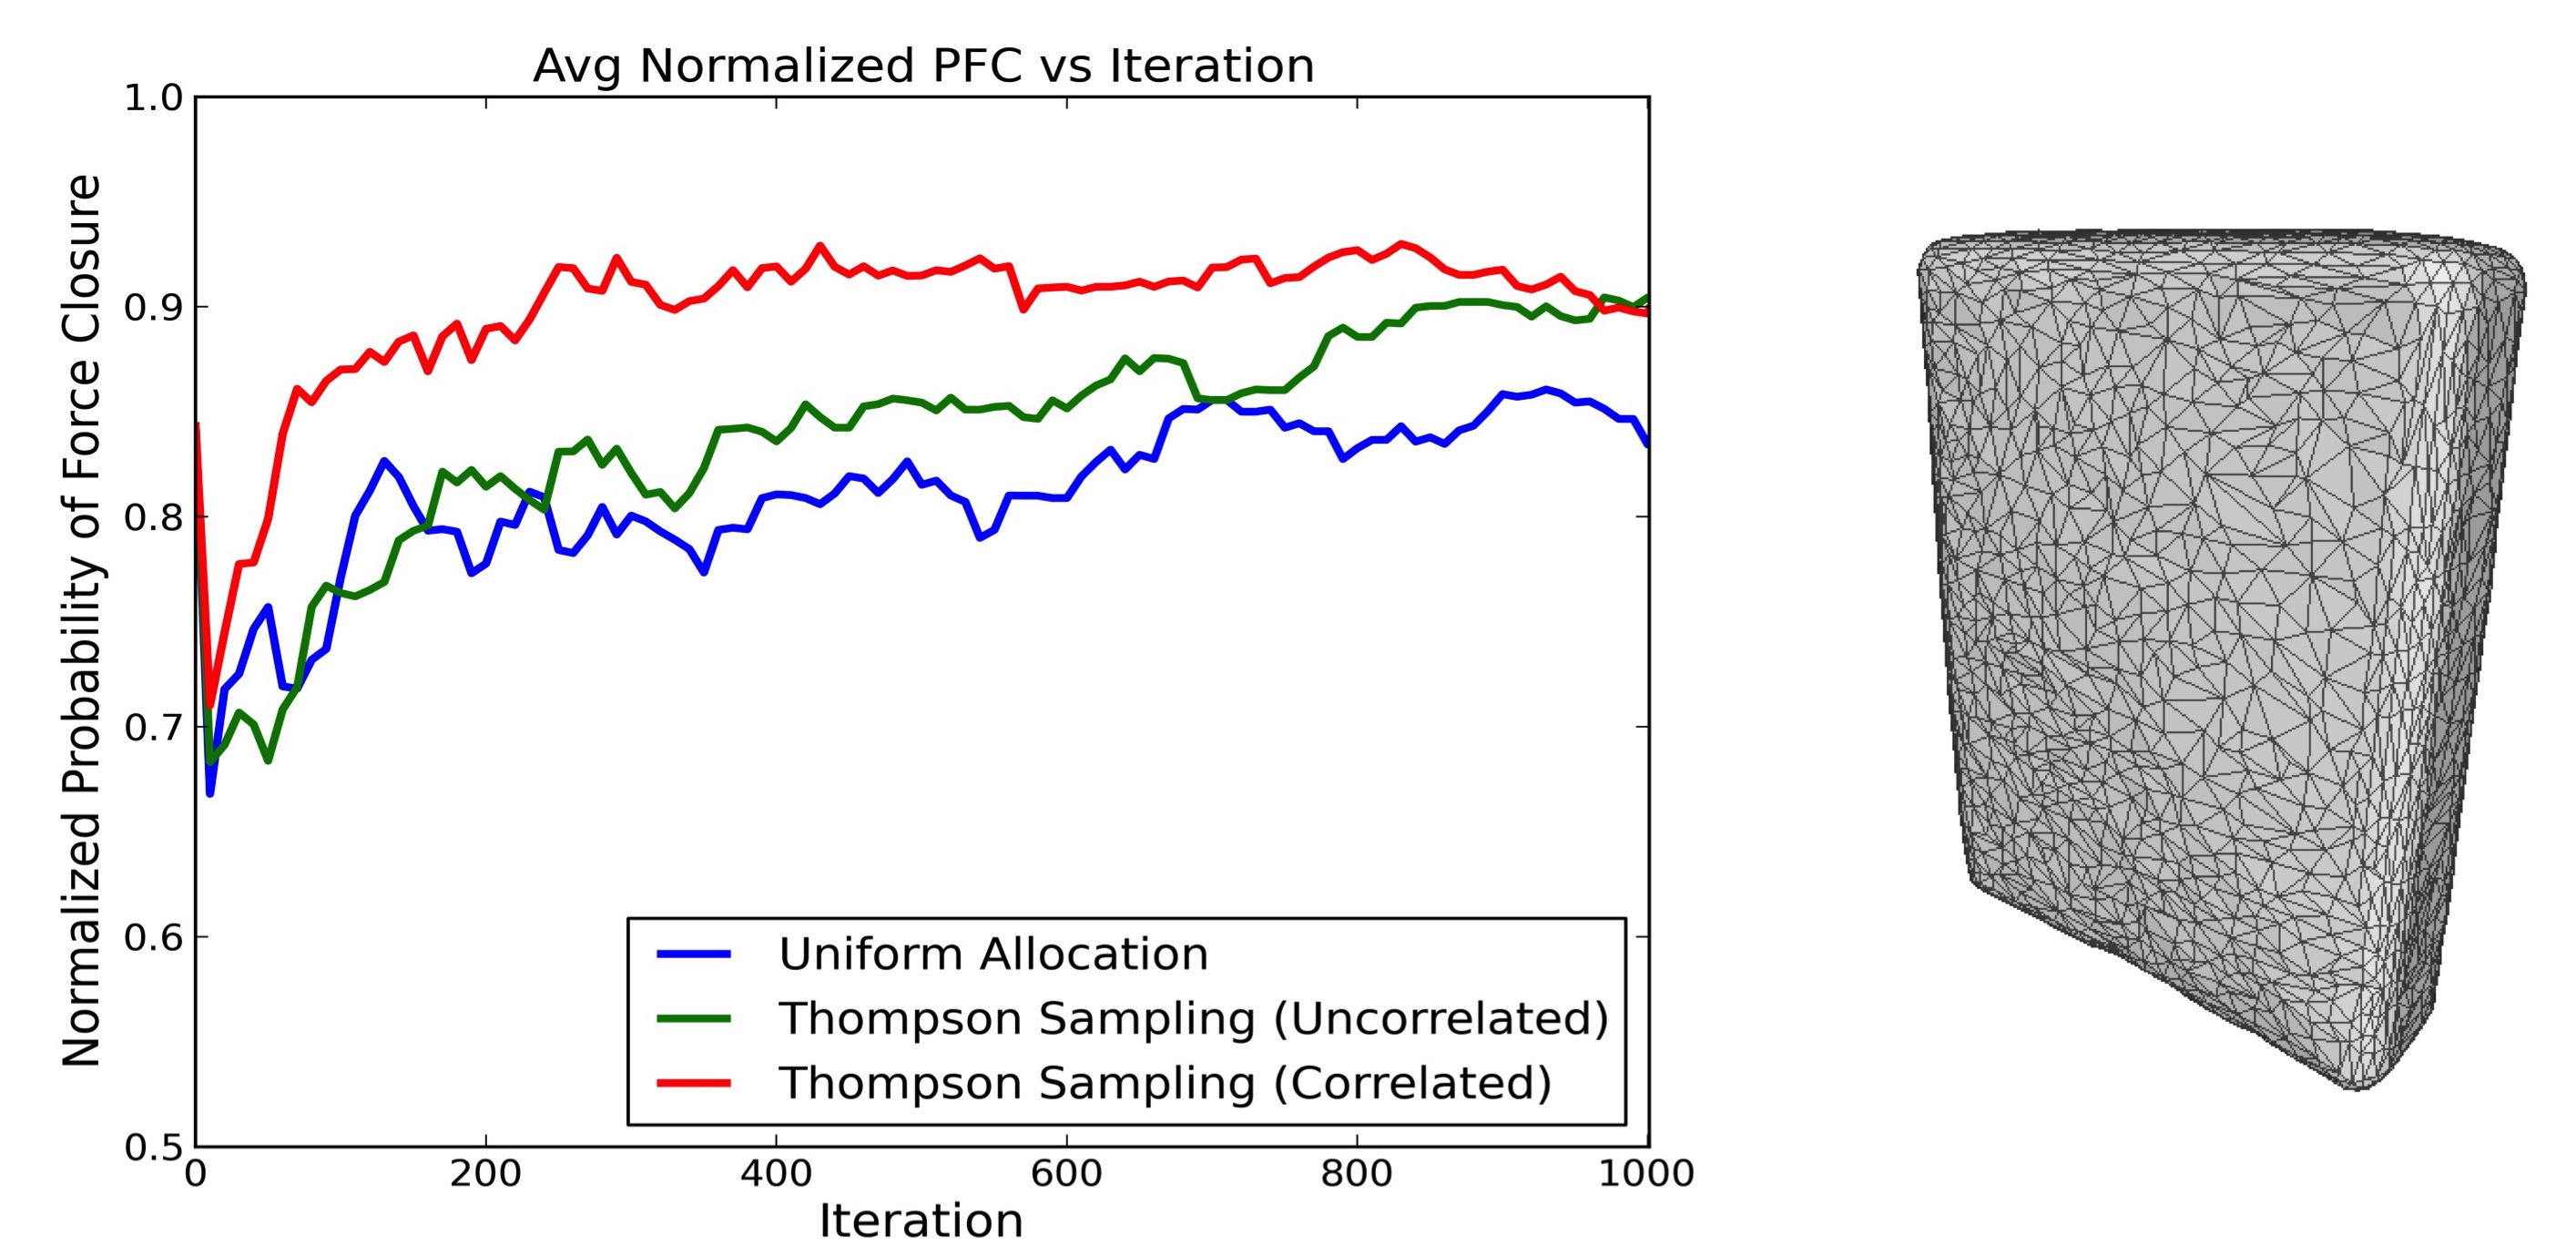
\includegraphics[scale=0.08]{figures/box_avg_reward_w_model.jpg}
        \caption{Normalized $P_F$ on a cereal box with 250 candidate grasps.}
    \end{subfigure}
    \begin{subfigure}[b]{0.5\textwidth}
        \centering
        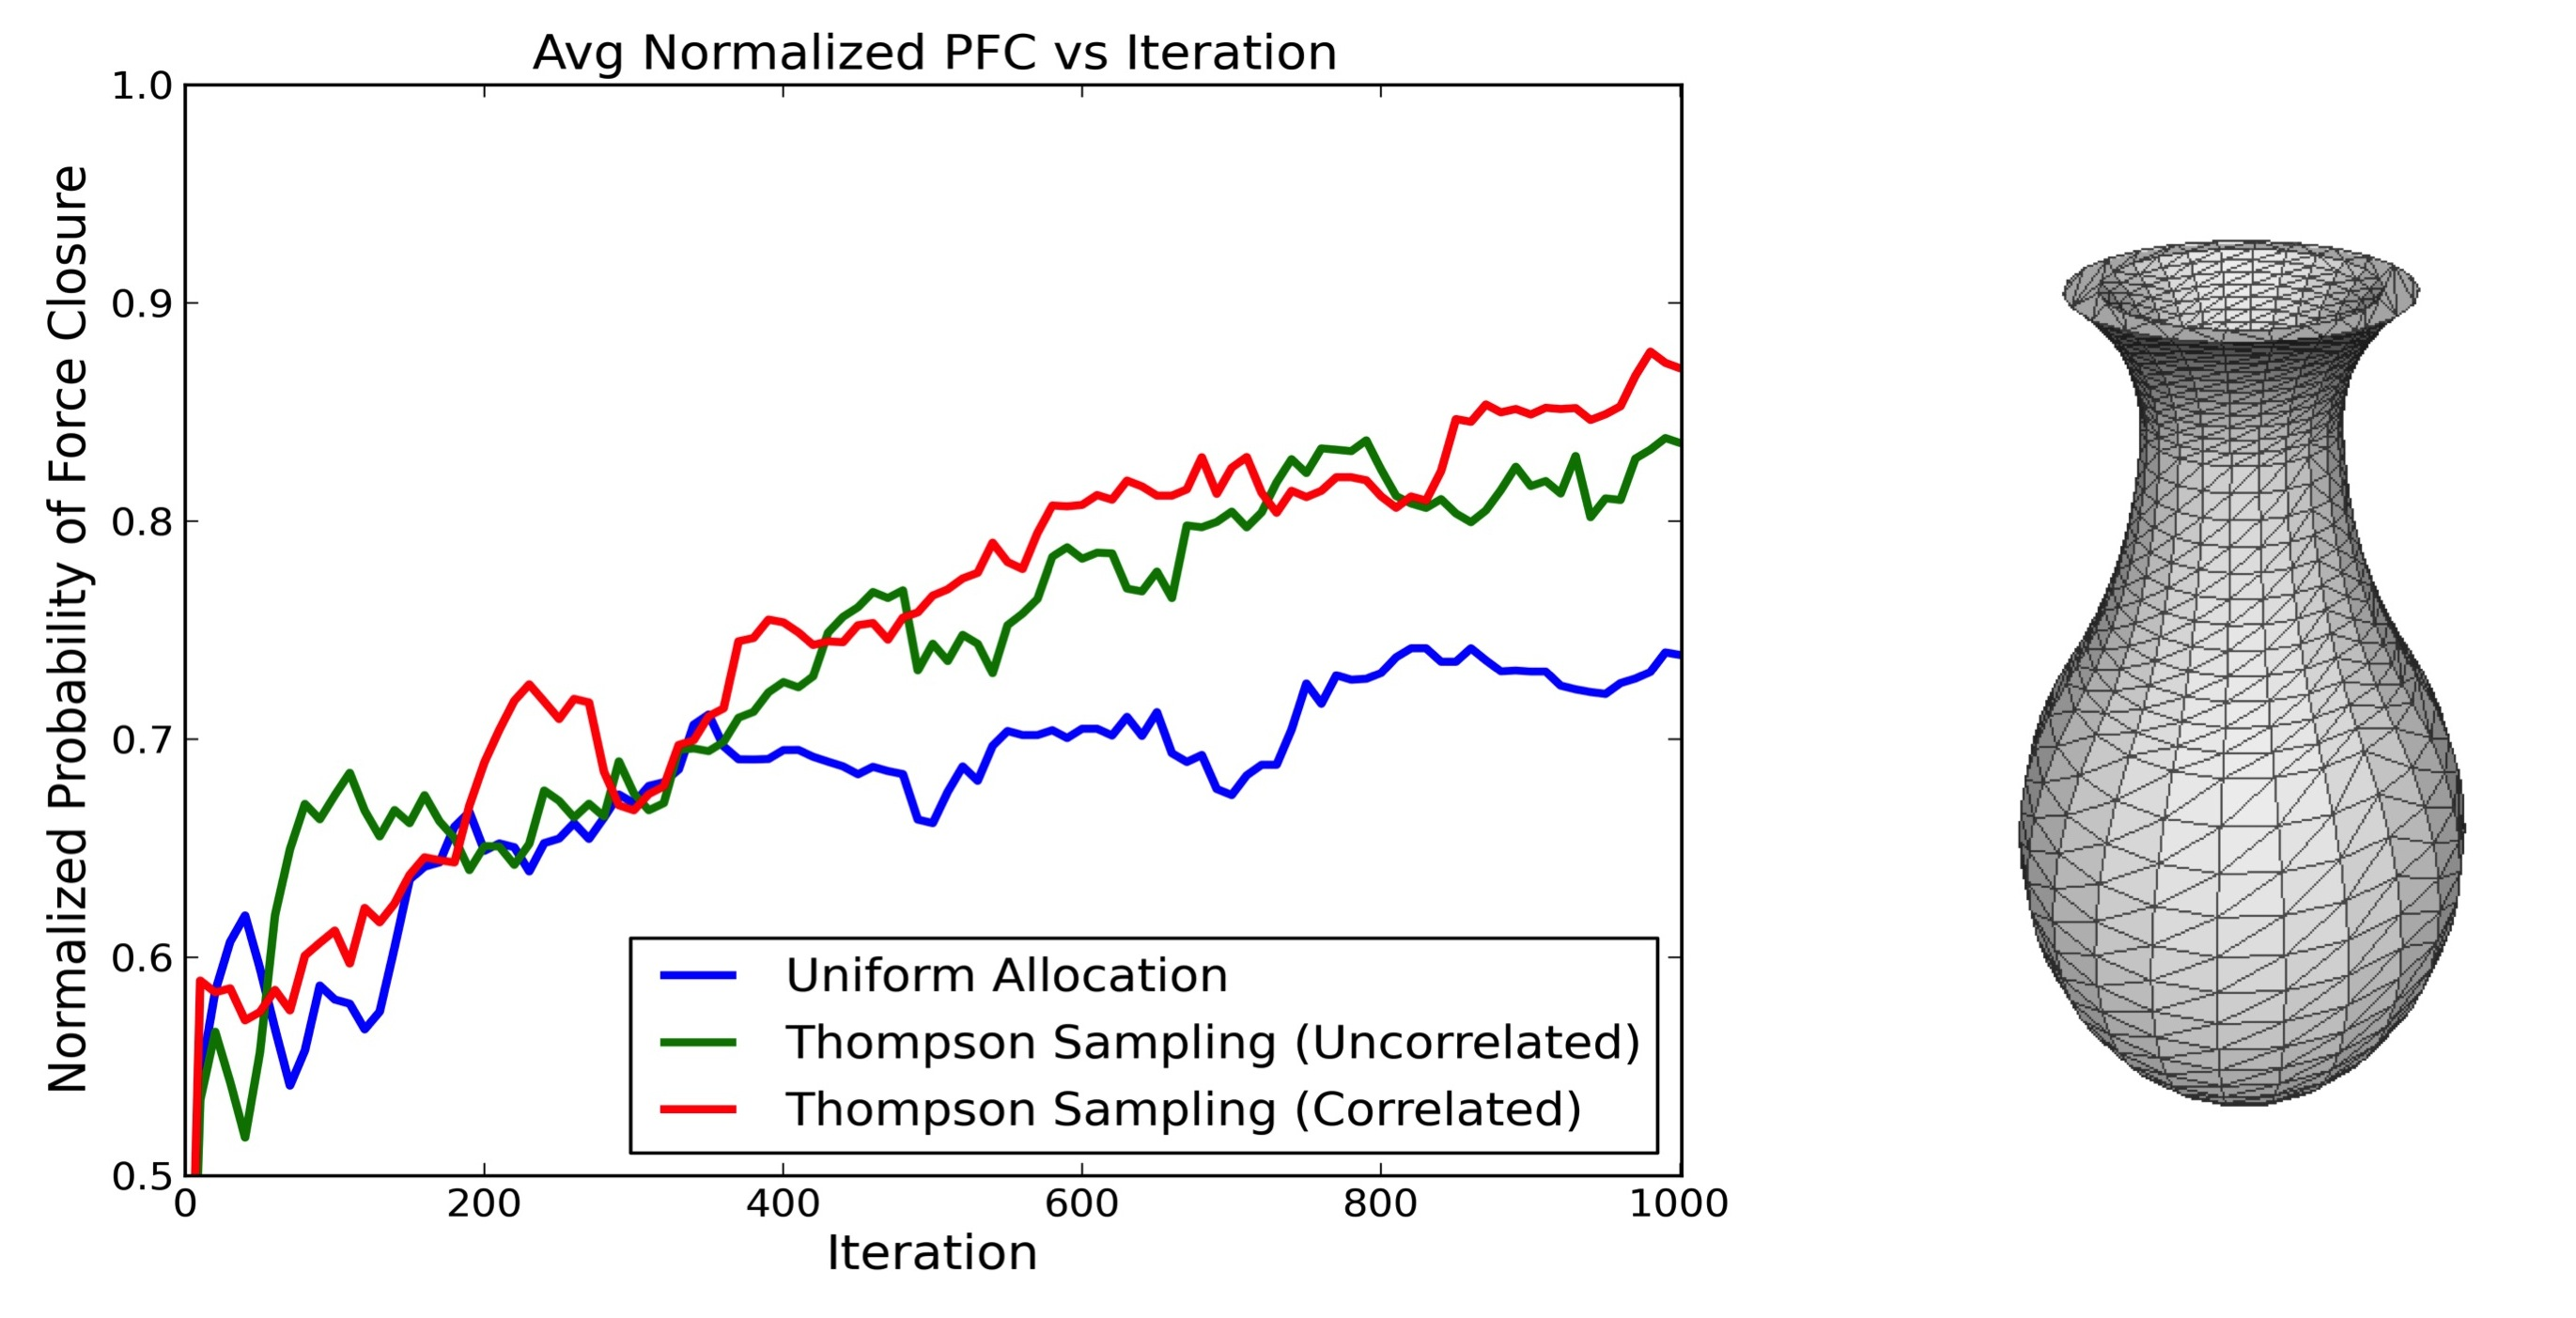
\includegraphics[scale=0.08]{figures/flowerpot_avg_reward_w_model.jpg}
        \caption{Normalized $P_F$ on a flower pot with 250 candidate grasps.}
    \end{subfigure}
\caption{Comparison of the normalized $P_F$ of the sampled grasp versus iteration of the MAB algorithm for correlated Thompson sampling, uncorrelated Thompson sampling, and Uniform Allocation averaged over 20 trials. (a) On the cereal box, correlated Thompson sampling converges to within 90\% of the highest quality grasp approximately 4$\times$ faster than uncorrelated. (b) However, correlated and uncorrelated Thompson sampling perform comparably on the flower pot because there are few grasp similarities in the candidate set. }
\figlabel{local-mab}
\vspace*{-15pt}
\end{figure}

To examine the effects of orders of magnitude of prior data in the MAB algorithms, we ran the algorithms with priors computed from increasingly larger subsets of prior data from DexNet: 0, 15, 150, and 1500 objects. 
\figref{global-mab} shows the normalized probability of force closure $P_F$ versus iteration when planning grasps for a bottle using prior grasp data from the five nearest neighbor objects in DexNet averaged over 50 trials.
Each other object was labelled with 250 grasps and $P_F$ evaluated using brute force Monte-Carlo integration.
We see that the convergence of the correlated MAB algorithms to a grasp with high $P_F$ accelerates with increasingly largers subsets of prior data used.
This suggests that adding more prior data may further accelerate convergence, because it is increasingly likely that a similar object and grasp exists in the dataset as the size increases.
Future work will examine these effects on a larger subset of objects and will use more than five nearest neighbors from DexNet to compute priors, which may lead to even larger gains for larger subsets of prior data.

\begin{figure}[t!]
\centering
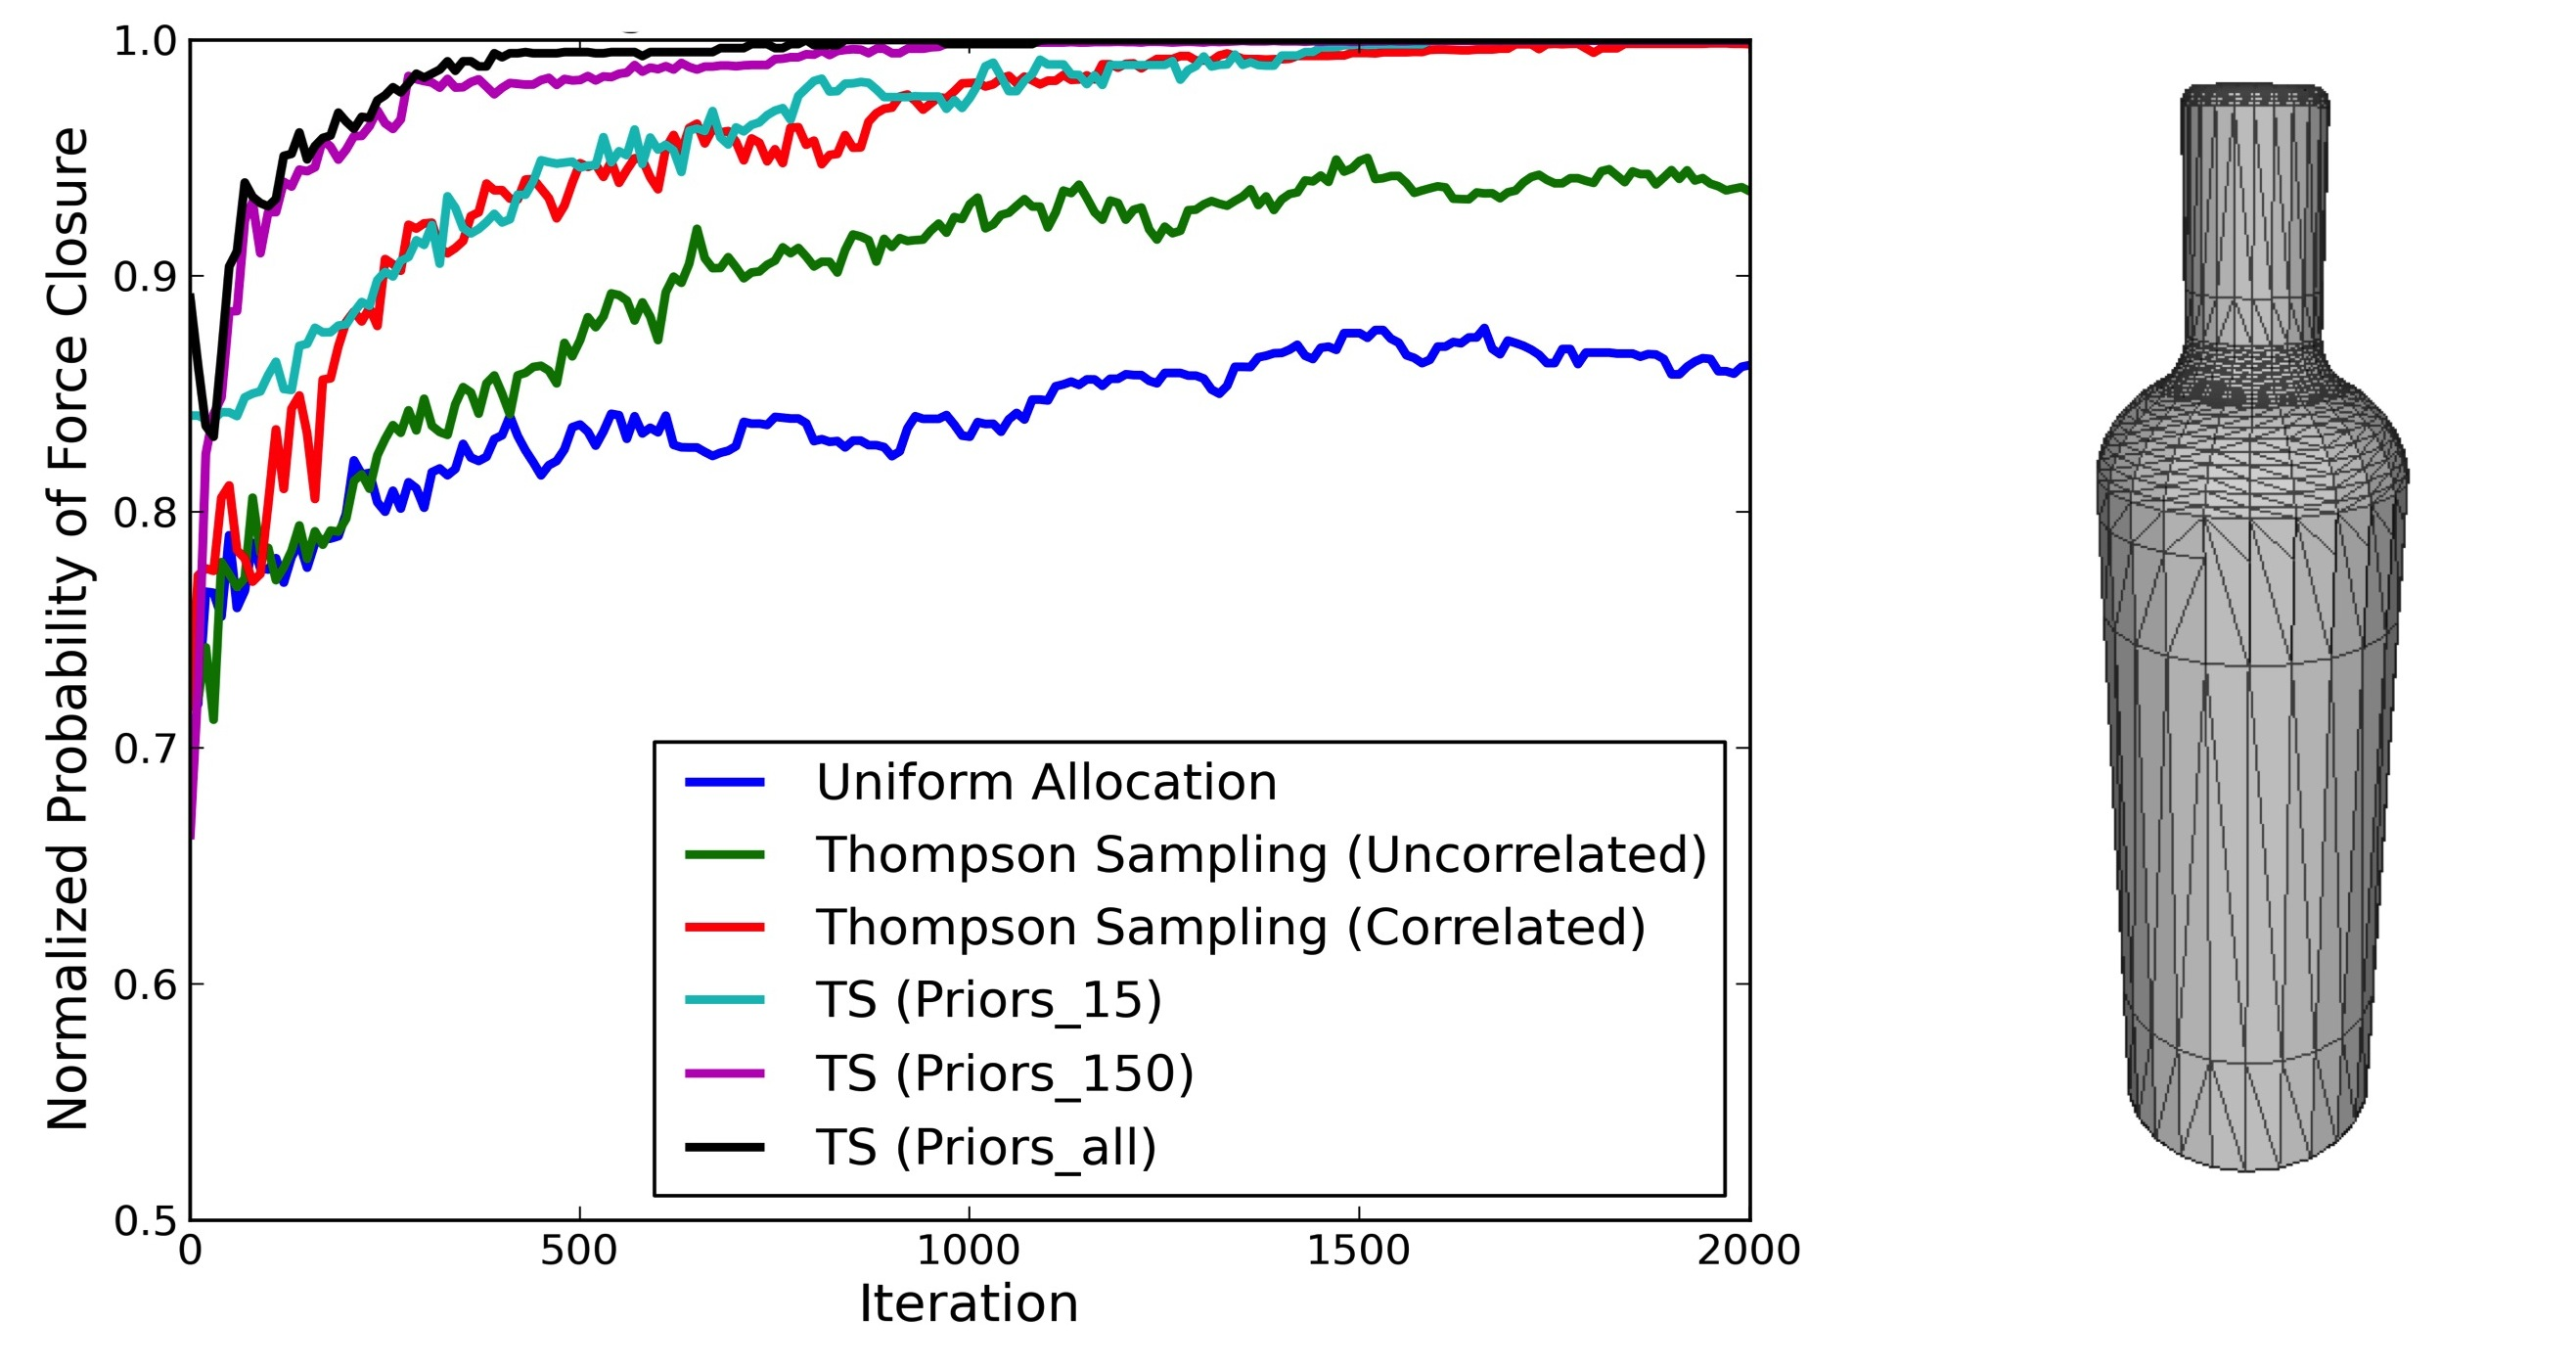
\includegraphics[scale=0.09]{figures/bottle_avg_reward_w_model2.jpg}
\caption{Comparison of the normalized $P_F$ of the sampled grasp (y-axis) versus iteration of the MAB algorithm (x-axis) for correlated Thompson sampling with and without the use of prior grasps from five nearest neighbors from DexNet, uncorrelated Thompson sampling, and Uniform Allocation averaged over 20 trials on the bottle object. Prior grasps were taken from increasingly larger subsets of DexNet: 15, 150, and 1500 objects. We see that convergence to within 90\% of the optimal grasp is accelerated by approximately 10$\times$ over uncorrelated Thompson sampling, and performance appears to improve with increasing sizes of the prior dataset used. }
\figlabel{global-mab}
\vspace*{-15pt}
\end{figure}

We are currently working on an experiment to quantify the gains in convergence time across orders of magnitudes of prior data (10, 100, 1000, 10000) from DexNet using Google Compute Engine.
Our initial version will be run on a relatively small subset of test objects, and in the coming weeks we will average the performance over a larger set of test objects.
We are particularly interested in seeing if there is a point of diminshing returns from adding more data when using datasets on the order of 10,000 - 100,000 objects.
We are also interested in whether or not adding perturbations to the data such as object reflections and shape perturbations will also increase performance, as has been observed for training Deep CNNs in vision~\cite{krizhevsky2012imagenet}.











%%\section{Introduction}
\seclabel{introduction}

Cloud-based Robotics and Automation systems exchange data and perform computation via networks instead of operating in isolation with limited computation and memory.
Potential advantages to using the Cloud include Big Data: access to updated libraries of images, maps, and object/product data; and Parallel Computation: access to parallel grid computing for statistical analysis, machine learning, and planning~\cite{kehoe2015survey}.
The advantages have recently been used in vision and speech, where datasets with millions of examples such as ImageNet have produced results~\cite{hannun2014deepspeech, krizhevsky2012imagenet} that surpass those obtained from decades of research on analytic methods.
This suggests that large-scale machine learning of grasps for vast numbers of possible object shapes, object poses, and environment configurations~\cite{goldfeder2011data, lenz2015deep, kappler2015leveraging}, could exhibit scaling effects similar to those observed in computer vision and speech recognition.

\begin{figure}[t!]
\centering
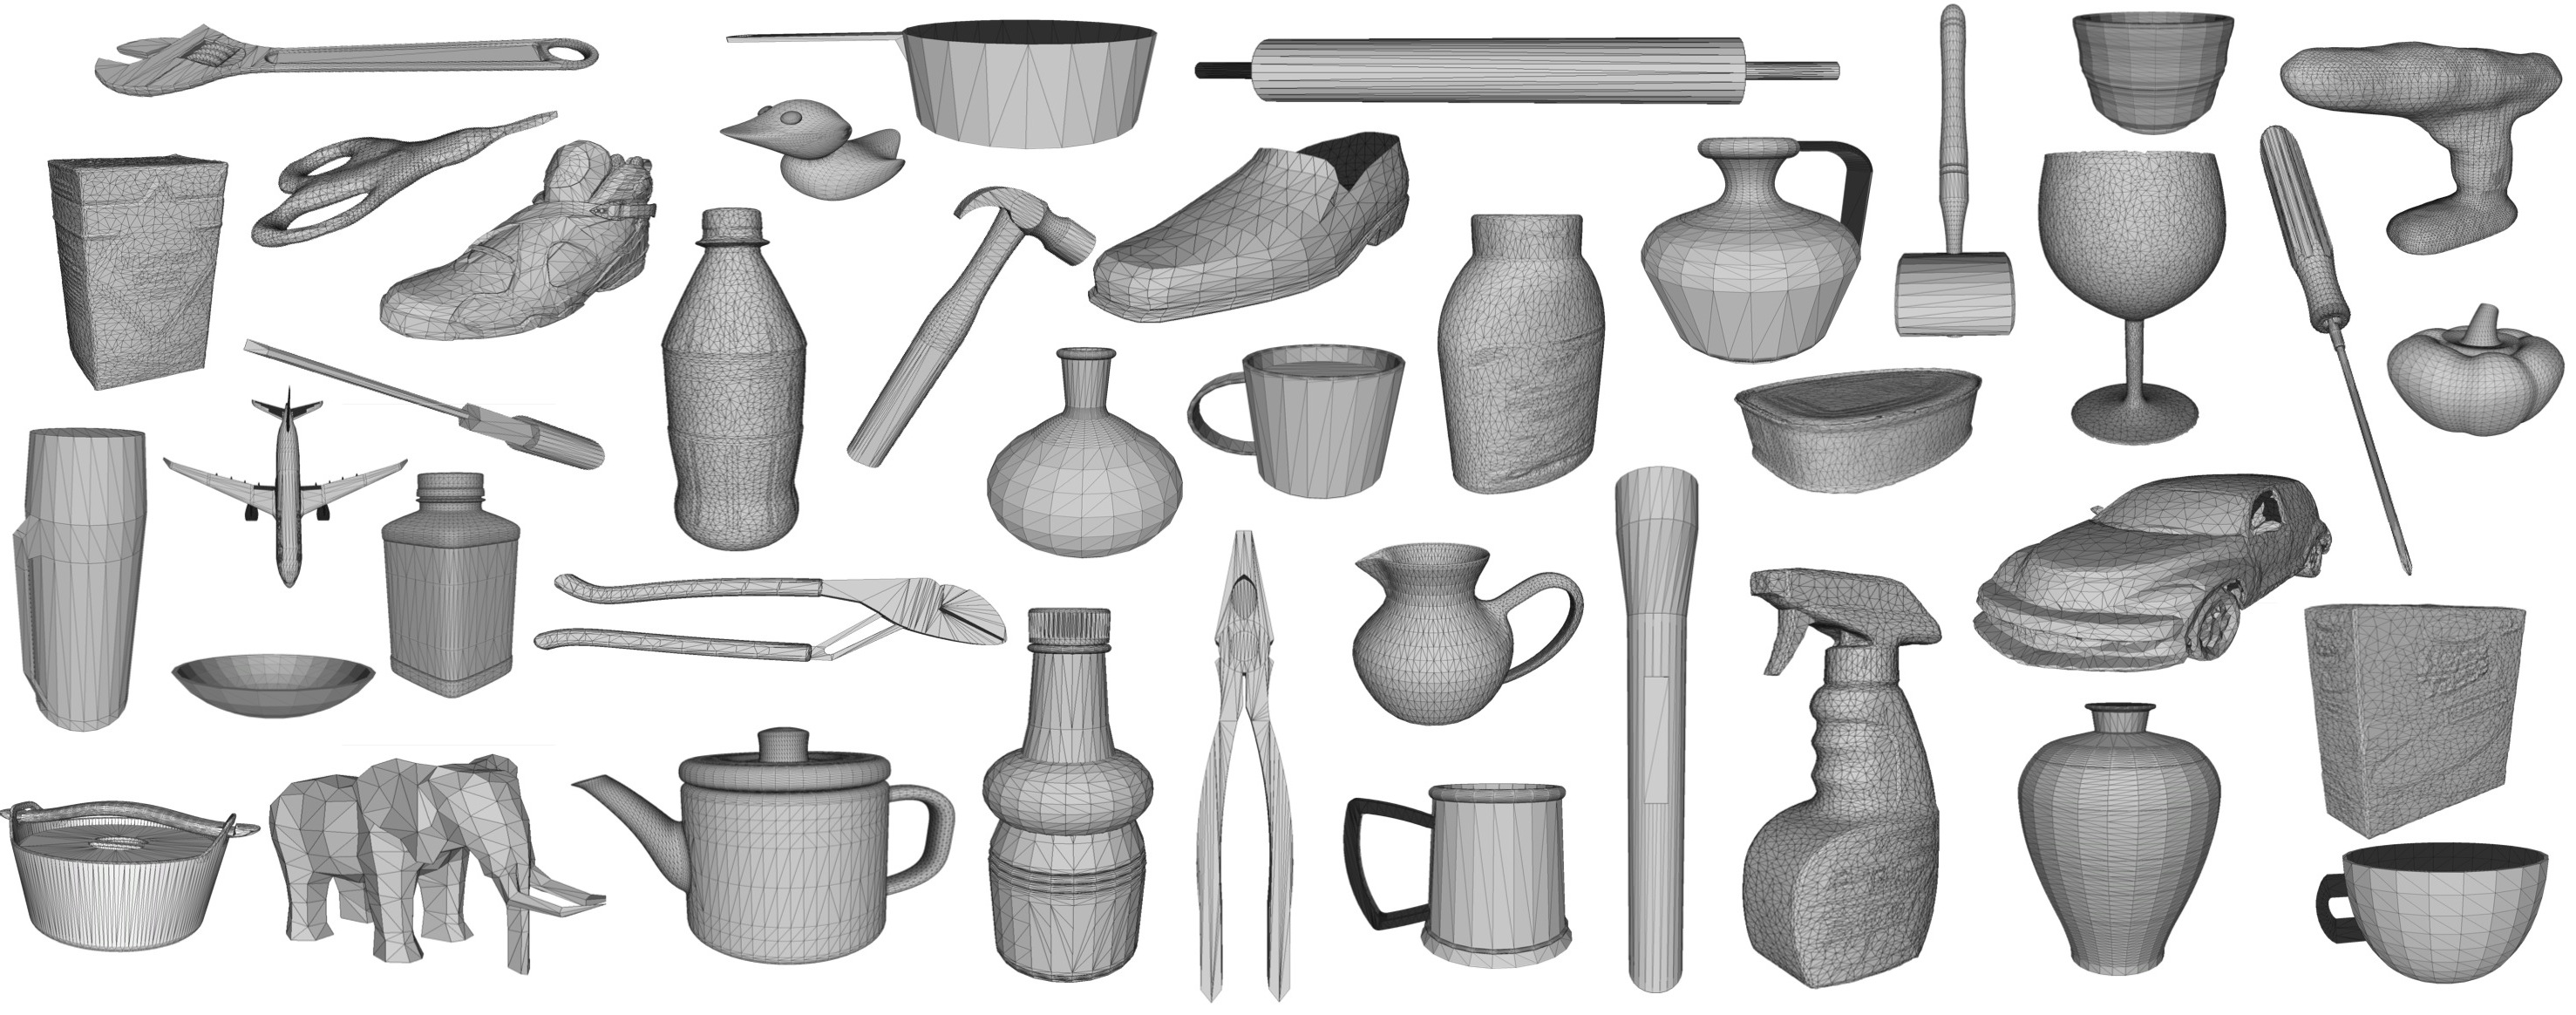
\includegraphics[scale=0.08]{figures/dexnet_collage.jpg}
\caption{Sample of 3D mesh models from the Dex-Net dataset that currently includes over 10,000 models from the KIT object database~\cite{kasper2012kit}, the Yale-CMU-Berkeley object set~\cite{calli2015benchmarking}, 3DNet\cite{wohlkinger20123dnet}, ModelNet~\cite{wu20153d}, and the SHREC 2014 object retrieval challenge dataset~\cite{li2015comparison}. }
\figlabel{dexnet-teaser}
\vspace*{-15pt}
\end{figure}

Our primary contribution is an algorithm based on a Multi-Armed Bandit (MAB) model with correlated rewards to speed up robust planning by learning from a large dataset of prior grasps and 3D object models.
Our algorithm is based on Continuous Correlated Beta Processes (CCBPs)~\cite{goetschalckx2011continuous, montesano2012active}, an efficient model for predicting a belief distribution on the quality of each grasp from prior data.

To study scaling effects we developed Dex-Net 1.0, a growing dataset that currently includes over 10,000 3D object models scaled to fit within a PR2 gripper and selected to reflect objects that could be encountered in warehousing or the home such as containers, tools, tableware, and toys.
~\figref{dexnet-teaser} shows a sample of the objects in the dataset.
%Dex-Net contains laser-scanned 3D mesh models from the KIT object database~\cite{kasper2012kit}, the Amazon Picking Challenge objects, BigBIRD~\cite{singh2014bigbird}, and YCB~\cite{calli2015benchmarking} to reflect physical objects commonly used for benchmarking in grasping research.
%The dataset also includes synthetic 3D mesh models from shape classification datasets such as 3DNet~\cite{wohlkinger20123dnet}, ModelNet~\cite{wu20143d}, and the SHREC 2014 large scale object retrieval challenge~\cite{li2015comparison} to approach larger scales.
Dex-Net also contains approximately 2.5 million parallel-jaw grasps, as each object is labelled with up to 250 grasps and an estimate of the probability of force closure for each under uncertainty in object pose, gripper pose, and friction coefficient.
To the best of our knowledge, this is the largest dataset used for grasping research to-date.
We also incorporate multi-view Convolutional Neural Networks (MV-CNNs)~\cite{su2015multi}, a state-of-the-art method for 3D shape classification, to efficiently retrieve similar 3D objects. 

We implement our algorithm on Google Compute Engine and store Dex-Net 1.0 on Google Cloud Storage, with a system that can run up to 1,500 instances at once.
Experiments on planning parallel-jaw grasps with high probability of force closure with our algorithm suggest that using 10,000 prior object models from Dex-Net can reduce the average number of samples needed to identify a grasp with high quality by $3.5\times$.
\TODO{Update with final results}

 






%\section{Related Work}
\seclabel{related}

For a survey of the substantial literature on grasping, see Prattichizzo and Trinkle~\cite{prattichizzo2008grasping}.
Research on grasp planning has focused on finding grasps by maximizing an analytic grasp quality metric based on wrench space (WS), such as the ability to resist external perturbations to the object based on the grasp WS~\cite{ferrari1992, miller2004graspit}, object WS~\cite{liu2015fast, pollard1994parallel}, or task WS~\cite{kruger2011partial, li1988task}.
WS metrics have been used to synthesize grasps for known objects using sampling-based optimization in software tools such as GraspIt!~\cite{miller2004graspit} or OpenGRASP~\cite{leon2010opengrasp}.
However, analytic WS metrics have been criticized~\cite{balasubramanian2012physical, weisz2012pose} for not being robust to variations in grasp acquistion, such as object shape, pose, material properties, and locations of contact~\cite{cheong2011output, diankov2010automated, weisz2012pose, zheng2005} and for not taking into account the dynamics of the the grasp~\cite{prattichizzo2008grasping}.
%This has motivated work on grasp transfer from a knowledge database to new objects, robust versions of analytic quality metrics with respect to uncertainty in the state of the robot and environment, and synthesis from statistical models of grasping learned from physical data or human labels.

The need to recompute WS metrics to select grasps for every new object motivated research on grasp synthesis by transferring grasps from a database of exemplar objects.
Li and Pollard~\cite{li2005shape} generated grasps by matching object shapes to human hand postured in a database.
Goldfelder et al.~\cite{goldfeder2009columbia} developed the Columbia grasp database, a database of 1,814 distinct models and over 200,000 force closure grasps generated using the Eigengrasp planner in GraspIt!~\cite{ciocarlie2009}.
The authors later used synthetic partial depth maps of objects in the database to match robot sensor data to precomputed grasps, using the Iterated Closest Point (ICP) algorithm to align the coordinate frames of the depth maps~\cite{goldfeder2009data, goldfeder2011data}.
Kehoe et al.~\cite{kehoe2013cloud} created a Cloud-based system to transfer grasps evaluated by probability of force closure on objects in a database to a physical robot by indexing the objects with the Google Goggles object recognition engine.
Recent research has also studied grasp transfer from objects of the same category by warping contacts betwen corresponding points on a shape surface and using local rigid alignment and contact interpolation~\cite{hillenbrand2012transferring, stouraitis2015functional} or by interpolating grasps and shapes over a vector space representation called a Grasp Moduli Space~\cite{pokorny2014grasp, pokorny2013grasp}.

Another line of research focused on making analytic grasp metrics robust to imprecision in perception and control~\cite{goldberg1990bayesian, stulp2011learning, zheng2005}.
Brook, Ciocarlie, and Hsiao~\cite{brook2011collaborative, hsiao2011bayesian} developed a Bayesian framework to evaluate both the expected epsilon quality and the probability of physical success on a PR2 given uncertainty in object identity, object pose, and gripper positioning on deterministic mesh and point cloud models. 
Weisz et al.~\cite{weisz2012pose} found that grasps ranked by probability of force closure subject to perturbations of object pose in simulation were empirically more successful on a physical robot than grasps planned using deterministic WS metrics. 
Kim et al.~\cite{kim2012physically} planned grasps using the expected epsilon quality metric~\cite{ferrari1992} under dynamics and uncertainty in pose, and found that the robust metric has a higher correlation with physical grasp success.
Recent research has also studied grasping under object shape uncertainty resulting from imprecision of object segmentations in images~\cite{christopoulos2007handling}, part tolerancing in manufacturing~\cite{kehoe2012estimating, kehoe2012toward, panahi2015orienting}, or missing and noisy data from depth sensors such as the Kinect modeled with Gaussian process implicit surfaces~\cite{dragiev2013uncertainty, mahler2015gp, laskey2015bandits}.
%Many have also studied caging gripper configurations~\cite{rimon1996caging}, which are a waypoint to form closure grasps for two fingers~\cite{vahedi2008caging, rodriguez2012caging} and may be robust to perturbations in object pose and shape~\cite{diankov2008manipulation, Wan2012_ICRA}.

Recent research has also studied synthesizing grasps by ranking grasps according statistical models learned from human annotations or physical execution~\cite{bohg2014data}.
Saxena et al.~\cite{jiang2011efficient, saxena2008robotic} used a logistic regression classified to predict grasp affordances in images from human annotated training data.
Lenz et al~\cite{lenz2015deep} used deep learning to detect bounding boxes for parallel-jaw grasps in color and depth images, which was extended to real time by Redmon and Angelova~\cite{redmon2014real}.
Herzog et al.~\cite{herzog2012template, herzog2014learning} extracted "heightmaps" of local object curvature from human demonstrated grasps, construct a library of heightmap templates, and match new sensor data to templates to select grasps similar to the demonstrations.
Detry et al.~\cite{detry2012generalizing} created a low-dimensional representation of object parts and cluster object parts that are grasped similarly to form a shape library of prototypical grasp parts, and show that this representation can be transferred to real sensor data~\cite{detry2013learning}.
Kappler et al.~\cite{kappler2015leveraging} trained a deep neural network to predict grasp success for a Barett hand measured by human annotations and the results of simulations on a database of synthetic pointclouds of objects.
Deep learning~\cite{krizhevsky2012imagenet} has also ben used in robotics for learning visuomotor policies for specific manipulation tasks~\cite{levine2015end} and recurrent control policies for cutting fruits vegetables from joint angles and end-effector forces~\cite{lenzdeepmpc}.
%Recently, several other works have proposed to form a huge database of grasps on synthetic objects from simulation outcomes~\cite{michalikg3db} or physical execution~\cite{tellex}.
In comparison, we learn a model to predict a Bayesian distribution on the probability of force closure for a grasp on an object based on similarity to a set of prior grasps and objects in a database, and use our model to actively decide the next grasp to evaluate using Multi-Armed Bandits.

Our work is also closely related to research on actively selecting grasps for building a statistical model of grasp quality from fewer examples.
Several works have searched for successful grasps using belief space planning to minimze uncertainty~\cite{hsiao2007grasping, kahnactive, fischinger2015learning}, but without use of an explicit grasp quality metric to guide the search.
Kehoe et al.~\cite{kehoe2012estimating} proposed iterative pruning, an algorithm for evaluating the probability of force closure for a set of candidate grasps while discrading grasps known to have poor quality.
Detry et al.~\cite{detry2011learning} estimated a full continuous density function over grasp poses using kernel density estimation and adaptively acquired samples by pruning unsuccessful grasps.
Kroemer et al.~\cite{kroemer2010combining} developed a reinforcement learning approach to grasp selection based on seeding hypotheses via imitation learning and Gaussian process upper-confidence bounds for active grasp acquisition.
Boularias et al.~\cite{boularias2014efficient, boularias2015learning} used a Gaussian process Bayesian Optimization model for selecting grasps on cluttered piles of rocks.
Salaganicoff et al.~\cite{salganicoff1996active} used active learning to decide the next grasp to execute on a physical robot while learning a predicitve model of empirical success from range sensors.
Similarly, Montesano and Lopes~\cite{montesano2012active} used Continuous Correlated Beta Processes~\cite{goetschalckx2011continuous} to actively acquire grasp executions on a physical robot, measuring correlations from the responses to a bank of image filters designed to detect grasp affordances such as edges.
Recently, Laskey et al.~\cite{laskey2015bandits} showed that Multi-Armed Bandit (MAB) algorithms can be used to accelerate the identification of grasps with high probability of force closure under uncertainty in shape, pose, and friction in 2D.
MAB algorithms trade off gaining information about grasps that have been sampled fewer times with exploiting the grasp with the highest estimated quality given the past samples.
In this work we extend the model of Laskey et al.~\cite{laskey2015bandits} to 3D and to utilize similarity between grasps across objects from Dex-Net with CCBPs to further reduce the number of samples needed to converge to a grasp with high quality.










%
%\section{Definitions and Problem Statement}
\seclabel{problem}

Let $g \in \mathfrak{se}(3)$ denote an attempted pose of the robot end-effector in 3D space, and $\Gamma = \{ g_1, ..., g_N\}$ denote a set of candidate grasps.
Let $\upsilon$ denote uncertainty in object shape represented by a Gaussian Process implicit surface~\cite{} distribution over signed distance fields $f$ with mean $\mu_f \in \mathbb{R}^{M \times M}$ and covariance $\Sigma_f$.
Let $\xi$ denote Gaussian uncertainty in object pose with mean $\mu_{\xi} \in \mathfrak{se}(3)$ and covariance $\Sigma_{\xi}$.
Let $\rho$ denote Gaussian uncertainty in gripper pose with mean $\mu_{\rho} \in \mathfrak{se}(3)$ and covariance $\Sigma_{\rho}$.
Let $\zeta$ denote Gaussian uncertiainty in friction coefficient mean $\mu_{\zeta} \in \mathbb{R}$ and covariance $\Sigma_{\zeta}$.

We are interested in finding the candidate grasp that maximizes the probability of force closure $P_F(g) = \mathbb{P} \left( F = 1 \big| g, \upsilon, \xi, \rho, \zeta\right)$~\cite{} subject to these sources of uncertainty over a budgeted maximum number of samples $T$.
To perform this as q	uickly as possible we formulate this as a maximization over the sum of $P_F$ for the grasps sampled at iteration $t$.

\vspace{-2ex}
\begin{align*}
	\maximum{g_1, ..., g_T \in \Gamma} \sum \limits_{t=1}^T P_F(g_{t})
\end{align*}

\noindent Laskey et al.~\cite{} proposed to solve this objective using algorithms for Multi-Armed Bandits.
In this work, we propose to use Multi-Armed Bandits with correlations between arms to further accelerate convergence.

%\section{Correlated Multi-Armed Bandit Model}
\seclabel{background}

Finding an approximate solution of Equation~\ref{eq:objective} using Multi-Armed Bandits requires a predictive model of the probability of force closure for each grasp.
We use Continuous Correlated Beta Processes (CCBPs) to model force closure for a grasp as a Bernoulli random variable with correlations across grasps and objects~\cite{goetschalckx2011continuous, montesano2012active}.
\figref{correlated-motivation} illustrates how using a correlated model can lead to accelerated convergence of bandit algorithms.
%In practice, correlations may occur between two grasps that contact the same shape in similar locations, or between grasps on different shapes, such as grasping the handle of a mug and the handle of a teapot.

\begin{figure}[t!]
\centering
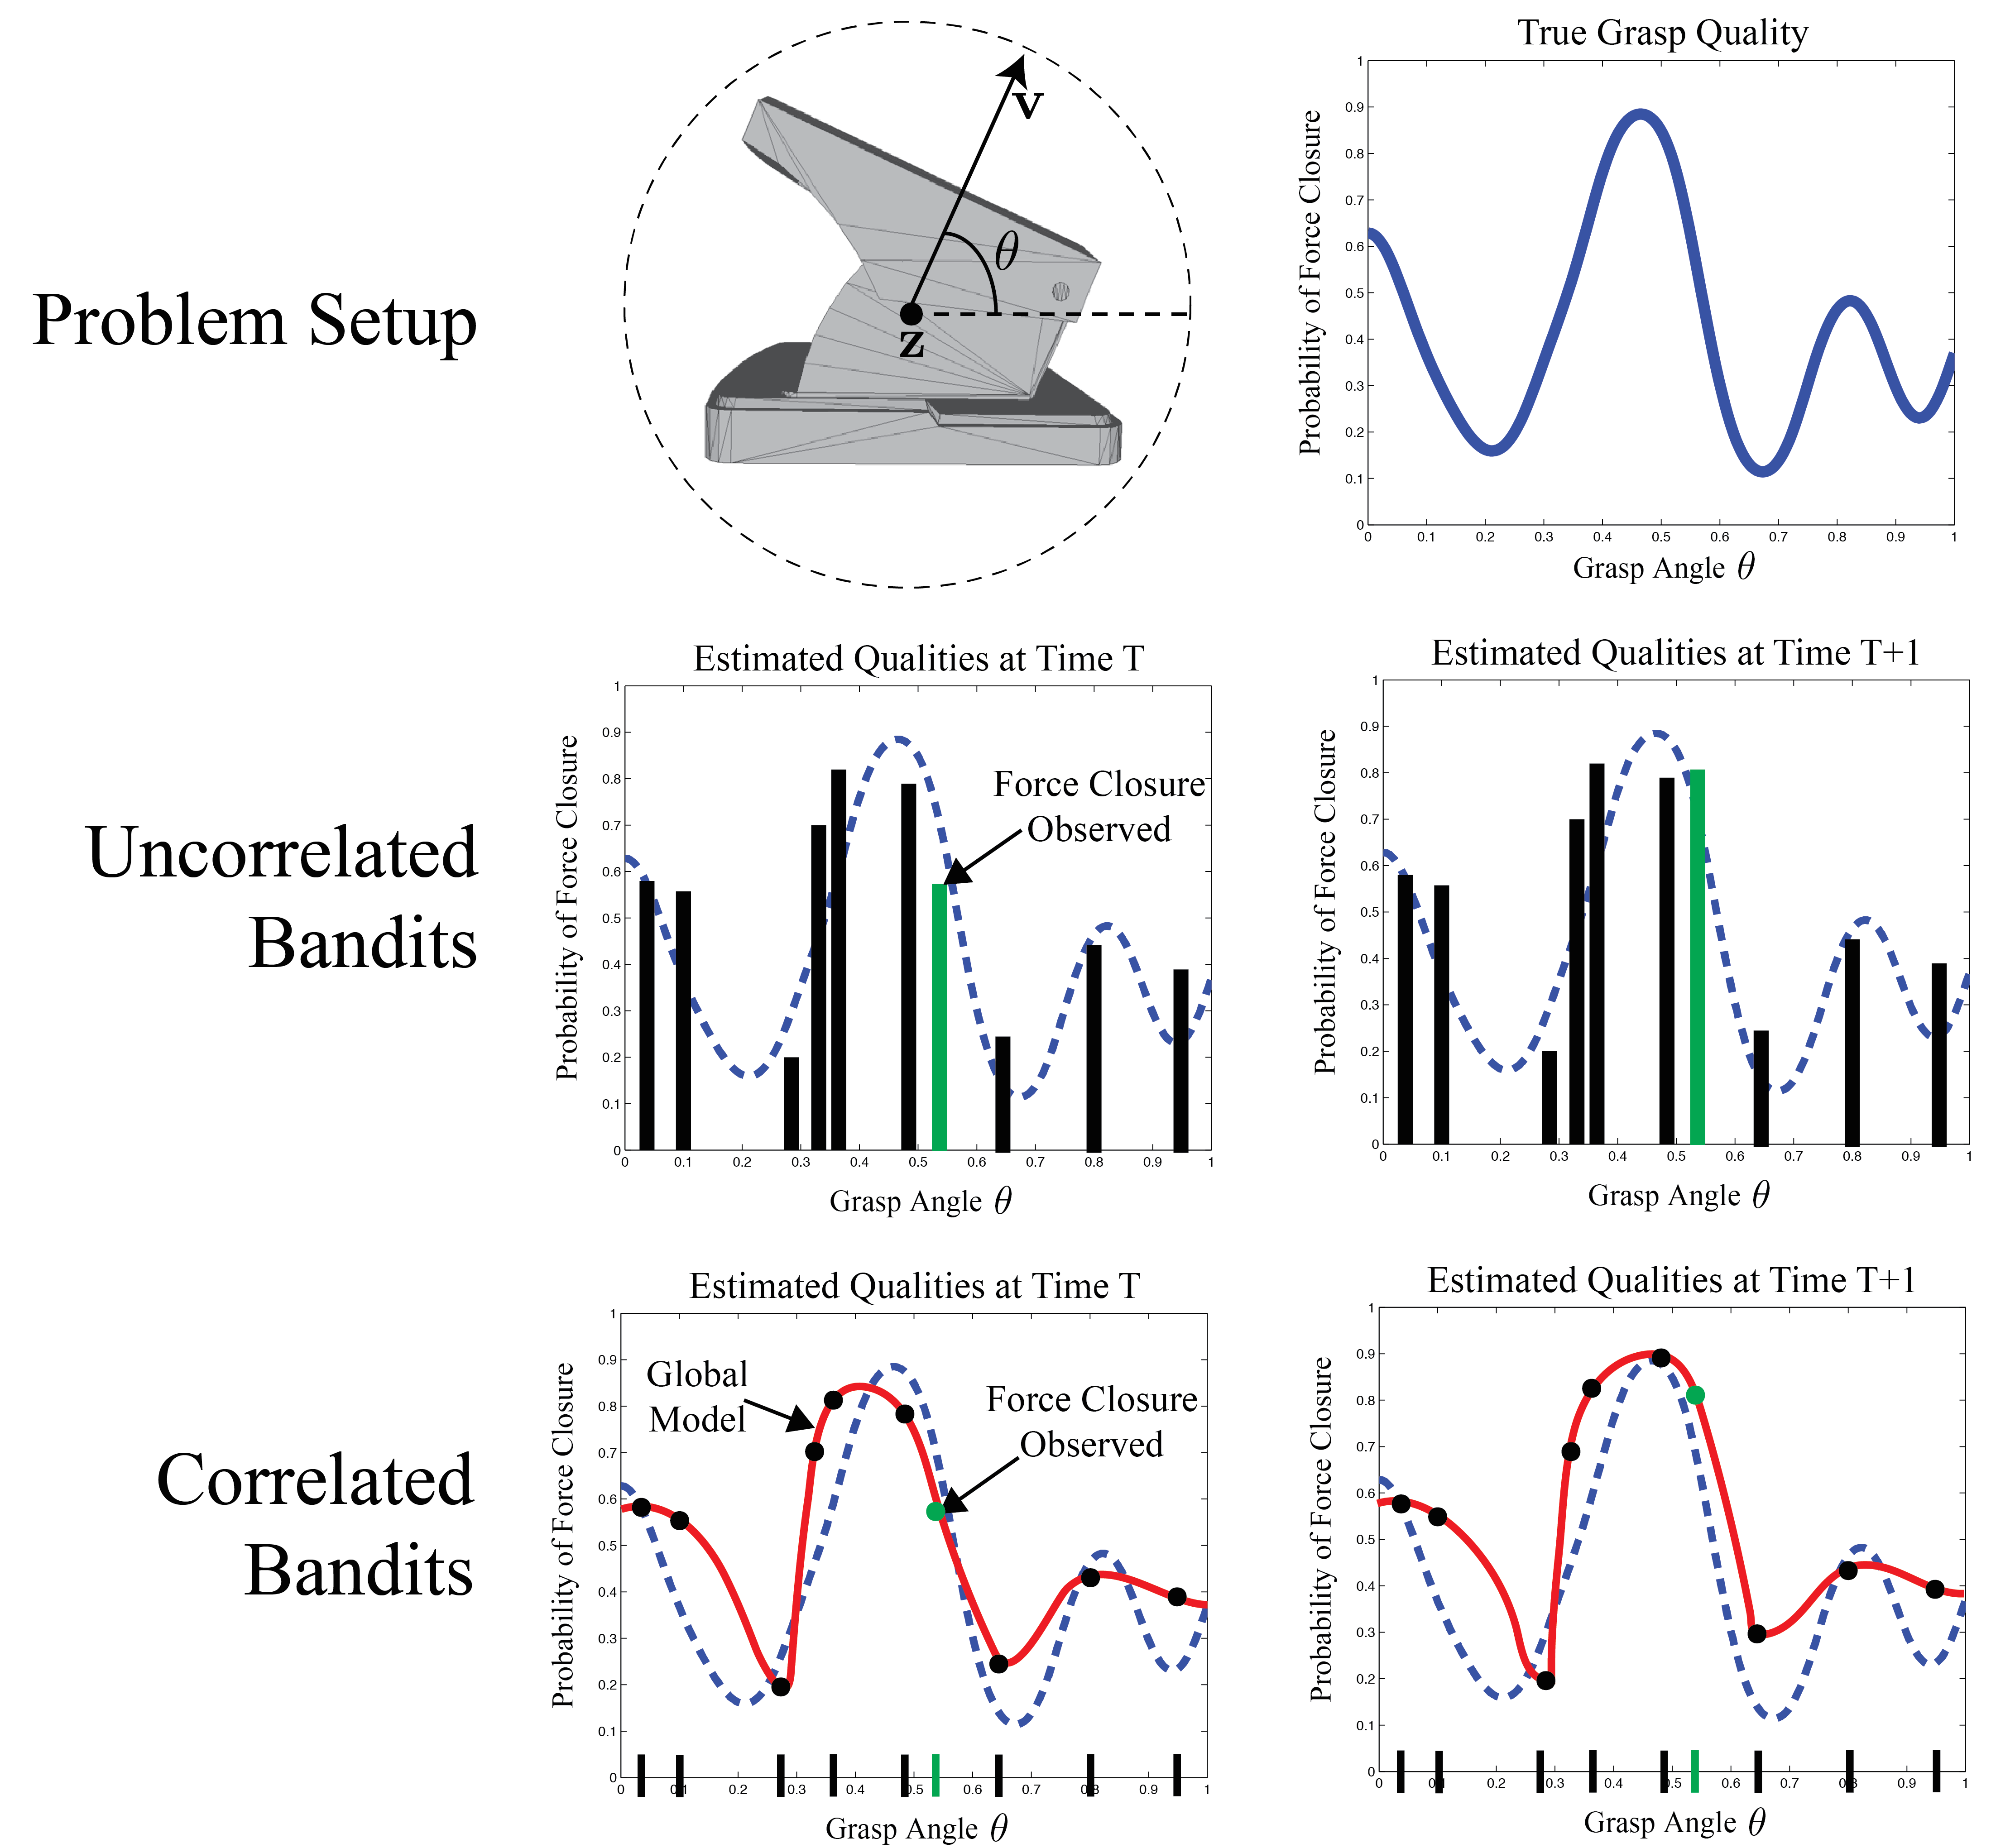
\includegraphics[scale=0.22]{figures/illustrations/correlated_bandits.png}
\caption{(Top Left) Consider a set of grasps with fixed center at an object center of mass and approach direction sampled along a one-dimensional circle. (Top Right) The true probability of force closure $P_F$ may vary smoothly as a function of the angle of the grasp axis. (Middle Left) Uncorrelated MAB models maintain an estimate of $P_F$ independently for each grasp, indicated by bars and their height. On iteration $T$ of a MAB algorithm, the grasp indicated with a green bar is sampled and returns force closure. (Middle Right) Only the estimate of $P_F$ for the sampled grasp is updated for iteration $T+1$, and the grasp with highest estimated $P_F$ remains suboptimal. (Bottom Left) Correlated MAB models maintain a global predictive function (in red) of $P_F$ for any possible grasp but may select grasps from a set of discrete candidates (indicated by dots). (Bottom Right) On iteration $T+1$ the grasp indicated by the green dot again returns force closure and the global model is updated, increasing the estimated $P_F$ for ``nearby" grasps. Although a suboptimal grasp was sampled, the global model now correctly predicts the optimal grasp in the set. }
\figlabel{correlated-model}
\vspace*{-15pt}
\end{figure}

\subsection{Continuous Correlated Beta Processes}

Continuous Correlated Beta Processes(CCBPs) were independently developed by Goetschalckx et al.~\cite{goetschalckx2011continuous} and Montesano and Lopes~\cite{montesano2012active} to model correlations between the Bernoulli random variables in a Beta-Bernoulli process, which may lead to faster convergence in Multi-Armed Bandit problems~\cite{chu2011contextual}.
Such correlations may exist when the Bernoulli random variables depend on common latent factors.
For example, two probability of force closure variables $\theta_k$ may be correlated when two grasps contact the same shape in similar locations or when grasps on different shapes have similar local surface geometries, such as grasping the handle of a mug and the handle of a teapot

Let $\Gamma = \{\bg_k\}_{k=1}^K$ denote our discrete set of $K$ candidate grasps for object $\mO$.
Let $F(\bg_k) \in \{0, 1\}$ denote the occurence of force closure for a grasp $\bg_k$.
We model $F(\bg_k)$ as a Bernoulli random variable with probability of success $\theta_k = P_F(\bg_k)$.
Since we do not know the value of $\theta_k$ for each grasp, we maintain a belief distribution for each $\theta_k$ based on our prior belief about the likelihood of force closure.
A common choice for a belief distribution on the Bernoulli parameter $\theta_k$ is the Beta distribution, which is specified by shape parameters $\alpha > 0$ and $\beta > 0$:

\vspace{-2ex}
\begin{align*}
	\betadist(\alpha, \beta) = \frac{1}{B(\alpha, \beta)} \theta_k^{\alpha-1} (1 - \theta_k)^{\beta-1}
\end{align*}

A CCBP estimates the shape parameters for a grasp $\bg$ on object $\mO$ using a normalized kernel function $k(\by_i, \by_j) : \mM \times \mM \rightarrow [0,1]$ that measures similarity between two elements of the Grasp Moduli Space, where $\by = \{\bg, \mO\} \in \mM$.
The kernel approaches 1 as the arguments become increasingly similar and approaches 0 as the arguments become dissimilar.
In this work we use a unit-bandwidth squared exponential kernel 
\begin{align*}
	k(\by_i, \by_j) &= \exp\left( - \frac{1}{2} \sum \limits_{m=1}^{N_f} w_m^2 \|\phi_m(\by_i) - \phi_m(\by_j)\|_2^2 \right)
\end{align*}
\noindent where $\phi_m: \mM \rightarrow \mathbb{R}^{d_m}$ for $m = 1, ..., N_f$ are feature mappings for a grasp and object to a $d_m$-dimensional Euclidean space and $w_m \in \mathbb{R}$ are weights scaling the relative contribution of the feature maps to the similarity metric.

Upon observing force closure for a grasp and object, we update the Beta belief for every other grasp proportional to how similar it is to the observed grasp as measured by the kernel. 
Let $F_{1}(\bg_{I(1)}), ..., F_{t}(\bg_{I(t)})$ be $t$ sequential observations of force closure from samples of our uncertainty models for grasps $\bg_{I(1)}, ..., \bg_{I(t)}$, where $I(j)$ is the index of the grasp sampled at time $j$.
Then the CCBP posterior update for $\theta_k$ is~\cite{goetschalckx2011continuous}:

\vspace{-2ex}
\begin{align}
	p \left(\theta_k | F_{1}(\bg_{I(1)}), ..., F_{t}(\bg_{I(t)}) \right) &= \betadist\left( \alpha_{k,t}, \beta_{k,t} \right) \notag \\
	\alpha_{k,t} = \alpha_{k,0} &+ \sum \limits_{j=1}^t k(\by_k, \by_{I(j)}) F_{i}(\bg_{I(j)}) \label{eq:alpha} \\
	\beta_{k,t} = \beta_{k,0} &+ \sum \limits_{=1}^t k(g\by_k, \by_{I(j)}) (1 - F_{i}(\bg_{I(j)})) \label{eq:beta}
\end{align}

\noindent Intuitively, this allows observations of one grasp to constitute fractional observations of similar grasps.

\subsection{Feature Mappings}
We use feature mappings $\phi_1, ..., \phi_{N_f}$ that capture both lsimilarity based on local surface geometry and grasp parameters and global object shape.

\subsubsection{Local Features}
Since grasps may be correlated across very small changes to the grasp center and approach direction on a single shape, our first feature map $\phi_{\ell}(\by) = \bg$ is the identity transformation for the grasp.
However, similarity between grasp centers and approach directions does not indicate similar $P_F$ if the two surfaces are dissimilar.
For example, two grasps contacting a box on opposite sides of a corner may be very similar according to $\phi_{\ell}$ but likely to contact the object on surfaces with very different orientations.

To mitigate this issue, we use a variant of the grasp heightmap features of Herzog et al.~\cite{herzog2012template} and Kappler et al.~\cite{kappler2015leveraging}.
In this work, we capture local surface patches by an image oriented along a tangent plane to the grasp axis at a contact point, where each pixel stores the distance from the pixel center on the plane to the surface along the grasp axis.
Let $d_g \in \mathbb{Z}$ be the number of pixels along each dimension of the heightmap, let $\delta \in \mathbb{R}$ be the resolution of the image pixels in meters, and let $r \in \mathbb{R}$ be a minimum projection distance.
Furthermore, let $\bc_k, k = 1, 2$ be a contact point for grasp $\bg$ and let $\bt_1, \bt_2$ be two orthogonal vectors to the grasp approach direction $\bv$.
Then to compute the heightmap value at pixel $(i,j)$ we first compute the 3D location of the pixel on the plane, $\bp_k(i,j) = \bc_k + i \delta \bt_1 + j \delta \bt_2$.
Then we assign the heightmap value $\bh_k(i,j) = t^*$, where $t^*$ is the smallest value of $t > -r$ such that $\bp_k(i,j) + t \bv$ contacts the shape surface.
Finally, we rotate the heightmap to align the axes with the eigenvectors of a weighted covariance matrix as in~\cite{tombariunique} in order to make our feature representation rotationally invariant.
Our feature vector for the heightmaps is $\phi_{h}(\bg_i, \mO_i) = [\bh_1, \bh_2]^T$.
\figref{local-feature-model} illustrates local surface patches extracted by this procedure.

\begin{figure}[t!]
\centering
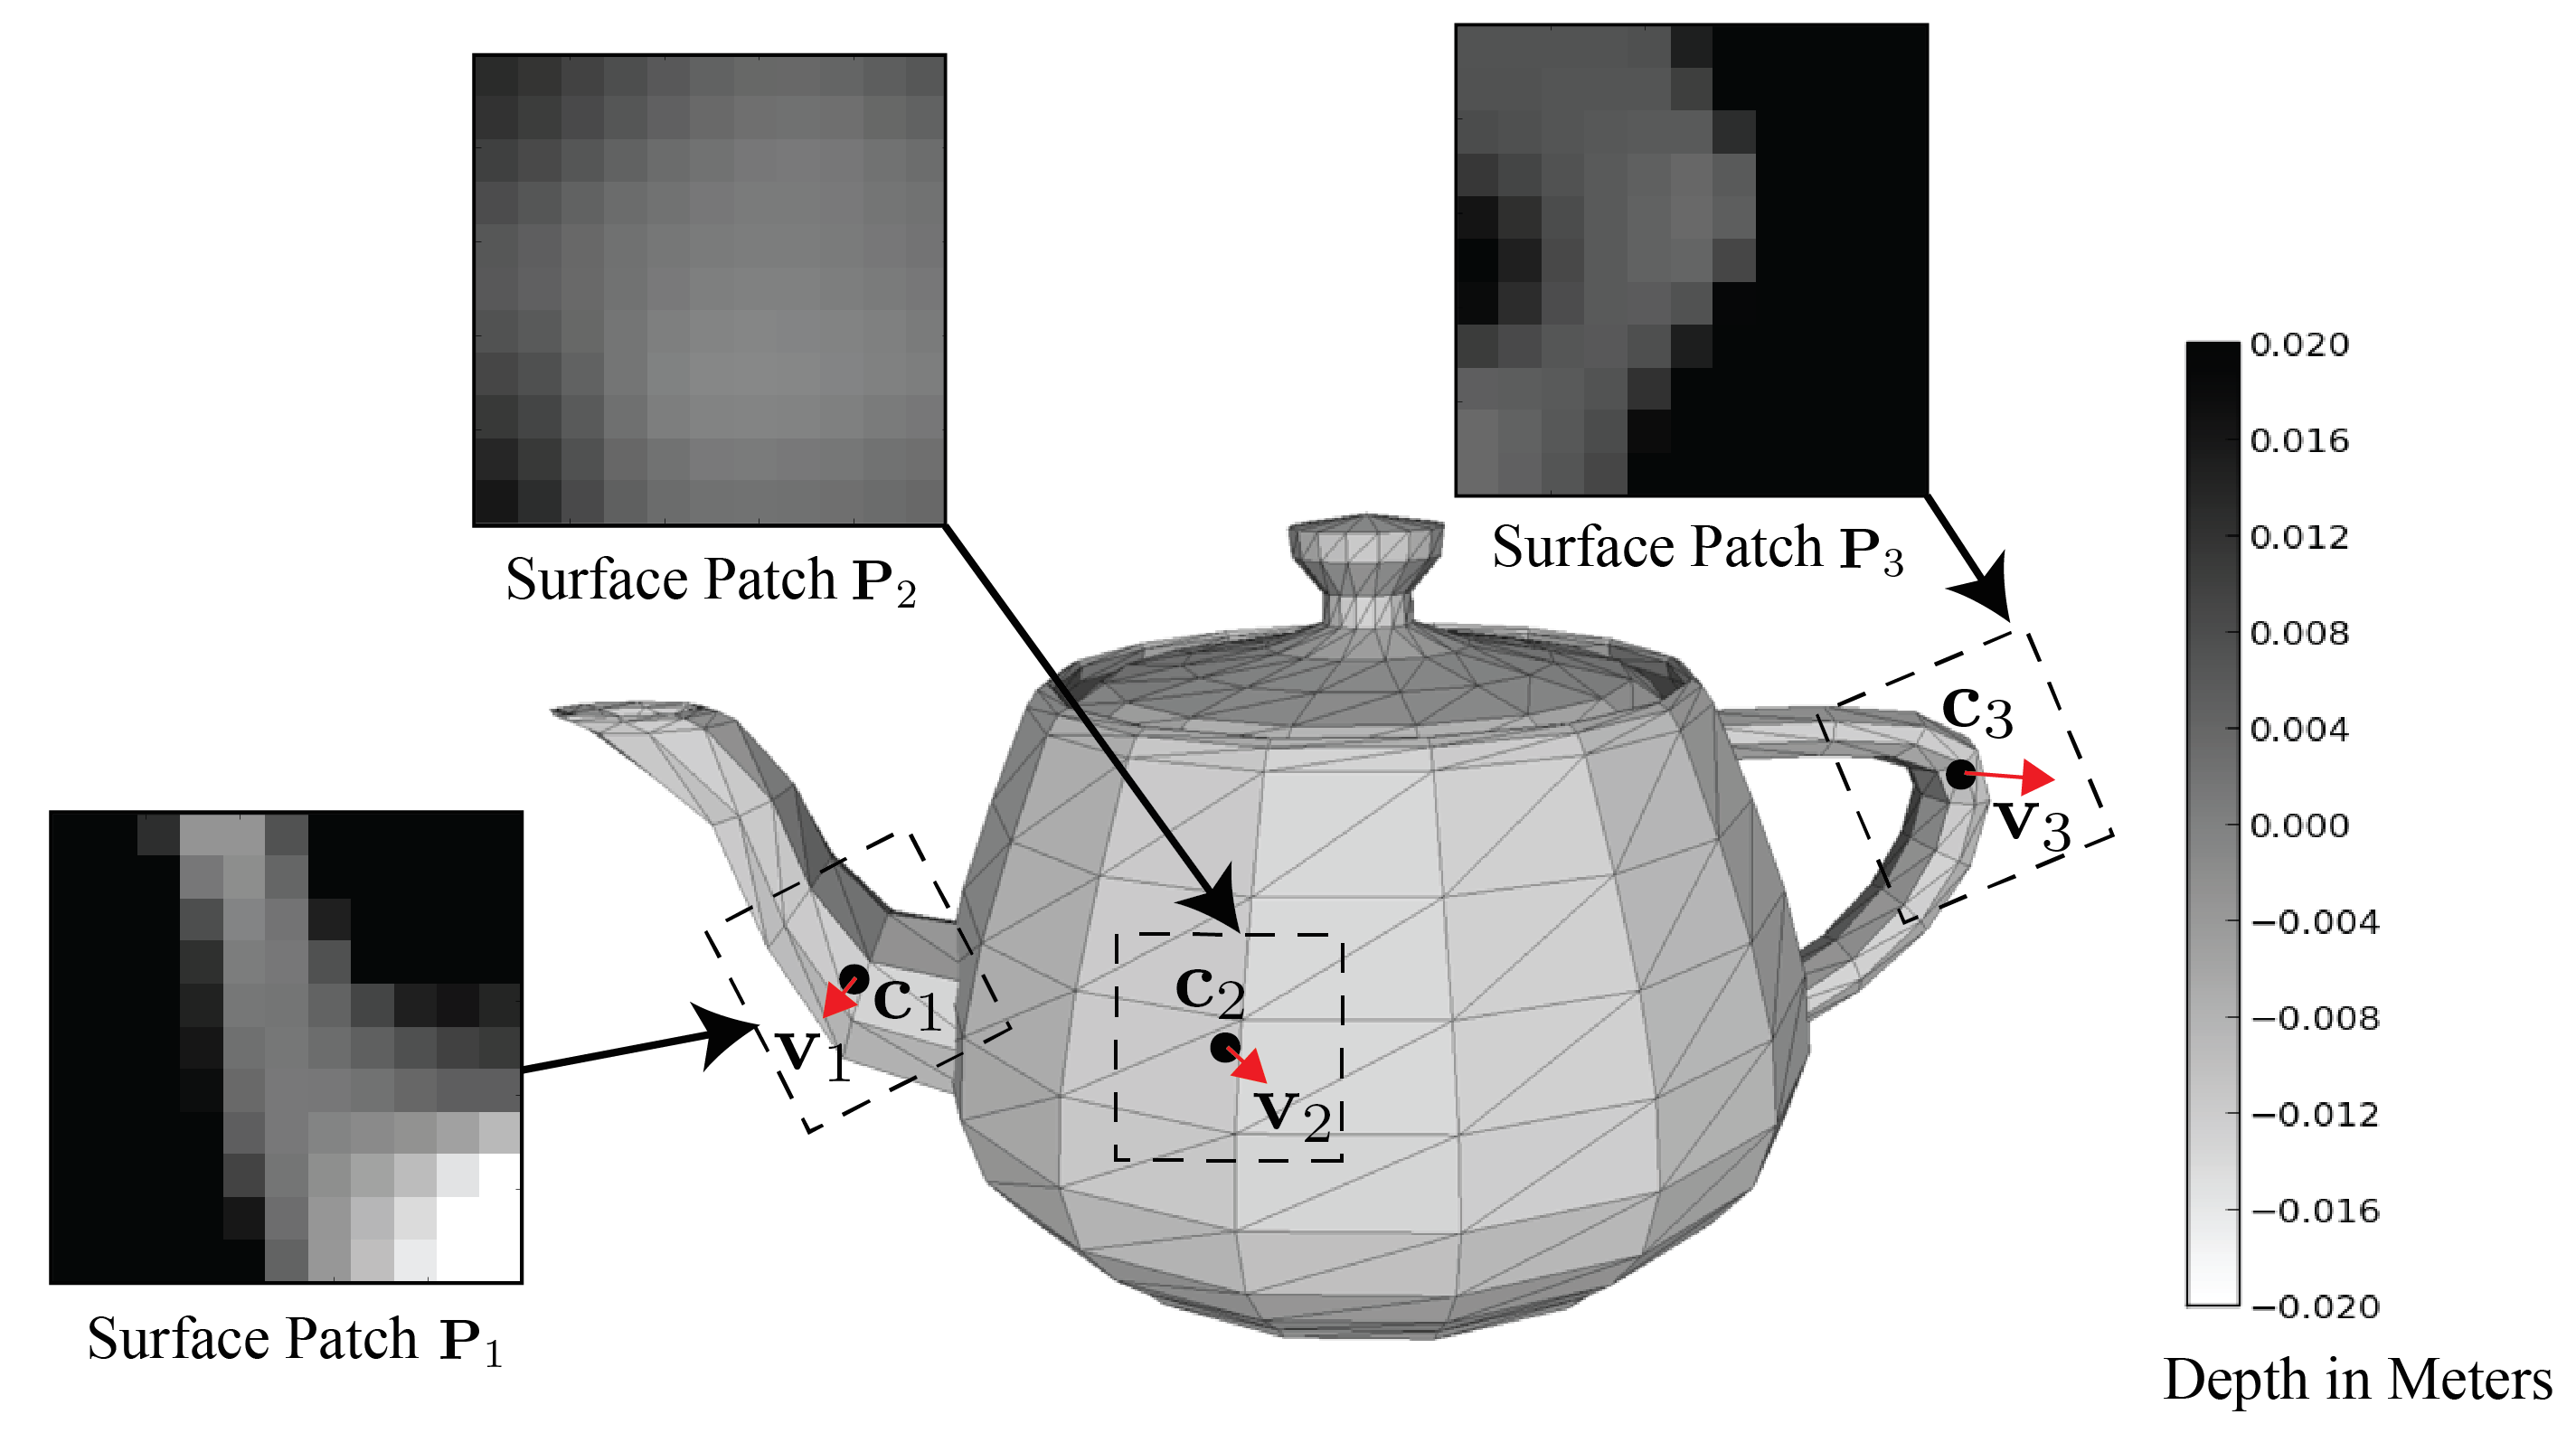
\includegraphics[scale=0.35]{figures/illustrations/local_feature_model.png}
\caption{Three local surface heightmaps extracted on a teapot. Each heightmap is ``rendered" along the grasp axis at each contact point and oriented by the local directions of maximum variation in the heightmap.  }
\figlabel{local-feature-model}
\vspace*{-15pt}
\end{figure}

\subsubsection{Global Features}
Purely local features may not capture all correlations in probability of force closure between pairs of grasps and objects.
For example, grasps on the handle of a teapot may have similar grasp center, grasp axis, and even local surface geometry to another tubelike object such as a pen, but different $P_F$.
To measure global shape similarity, we develop a novel viewpoint-based object representation that pools the views from many virtual viewpoints rendered on a sphere surrounding the object.

\TODO{Justify why class labels help, if they do}
\figref{global-feature-model} illustrates our method.
We first render every object to 50 virtual cameras discretized along equal angle increments and oriented toward the object center using Maya.
Then we finetune AlexNet~\cite{krizhevsky2012imagenet}, a common deep Convolutional Neural Network (CNN) architecture, to predict a class label for each image based on known class labels for the 3D models.
%While class labels are not necessarily indicative of similarity in the geometry relevant to grasping, in many cases the same class label is enough to guarantee some correspondence of global geometry.
Next, we pass each of the 50 views of each object through the finetuned CNN and max-pool the output of the fc7 layer.
As the output is nearly 400 dimensions, we finally reduce the max-pooled output to 100 dimensions using Principal Component Analysis (PCA).
This yields a representation $\psi(\mO) \in \mathbb{R}^{100}$ for each object.

\TODO{Expand above paragraph, include more details on method as well as the results of training}

\begin{figure}[t!]
\centering
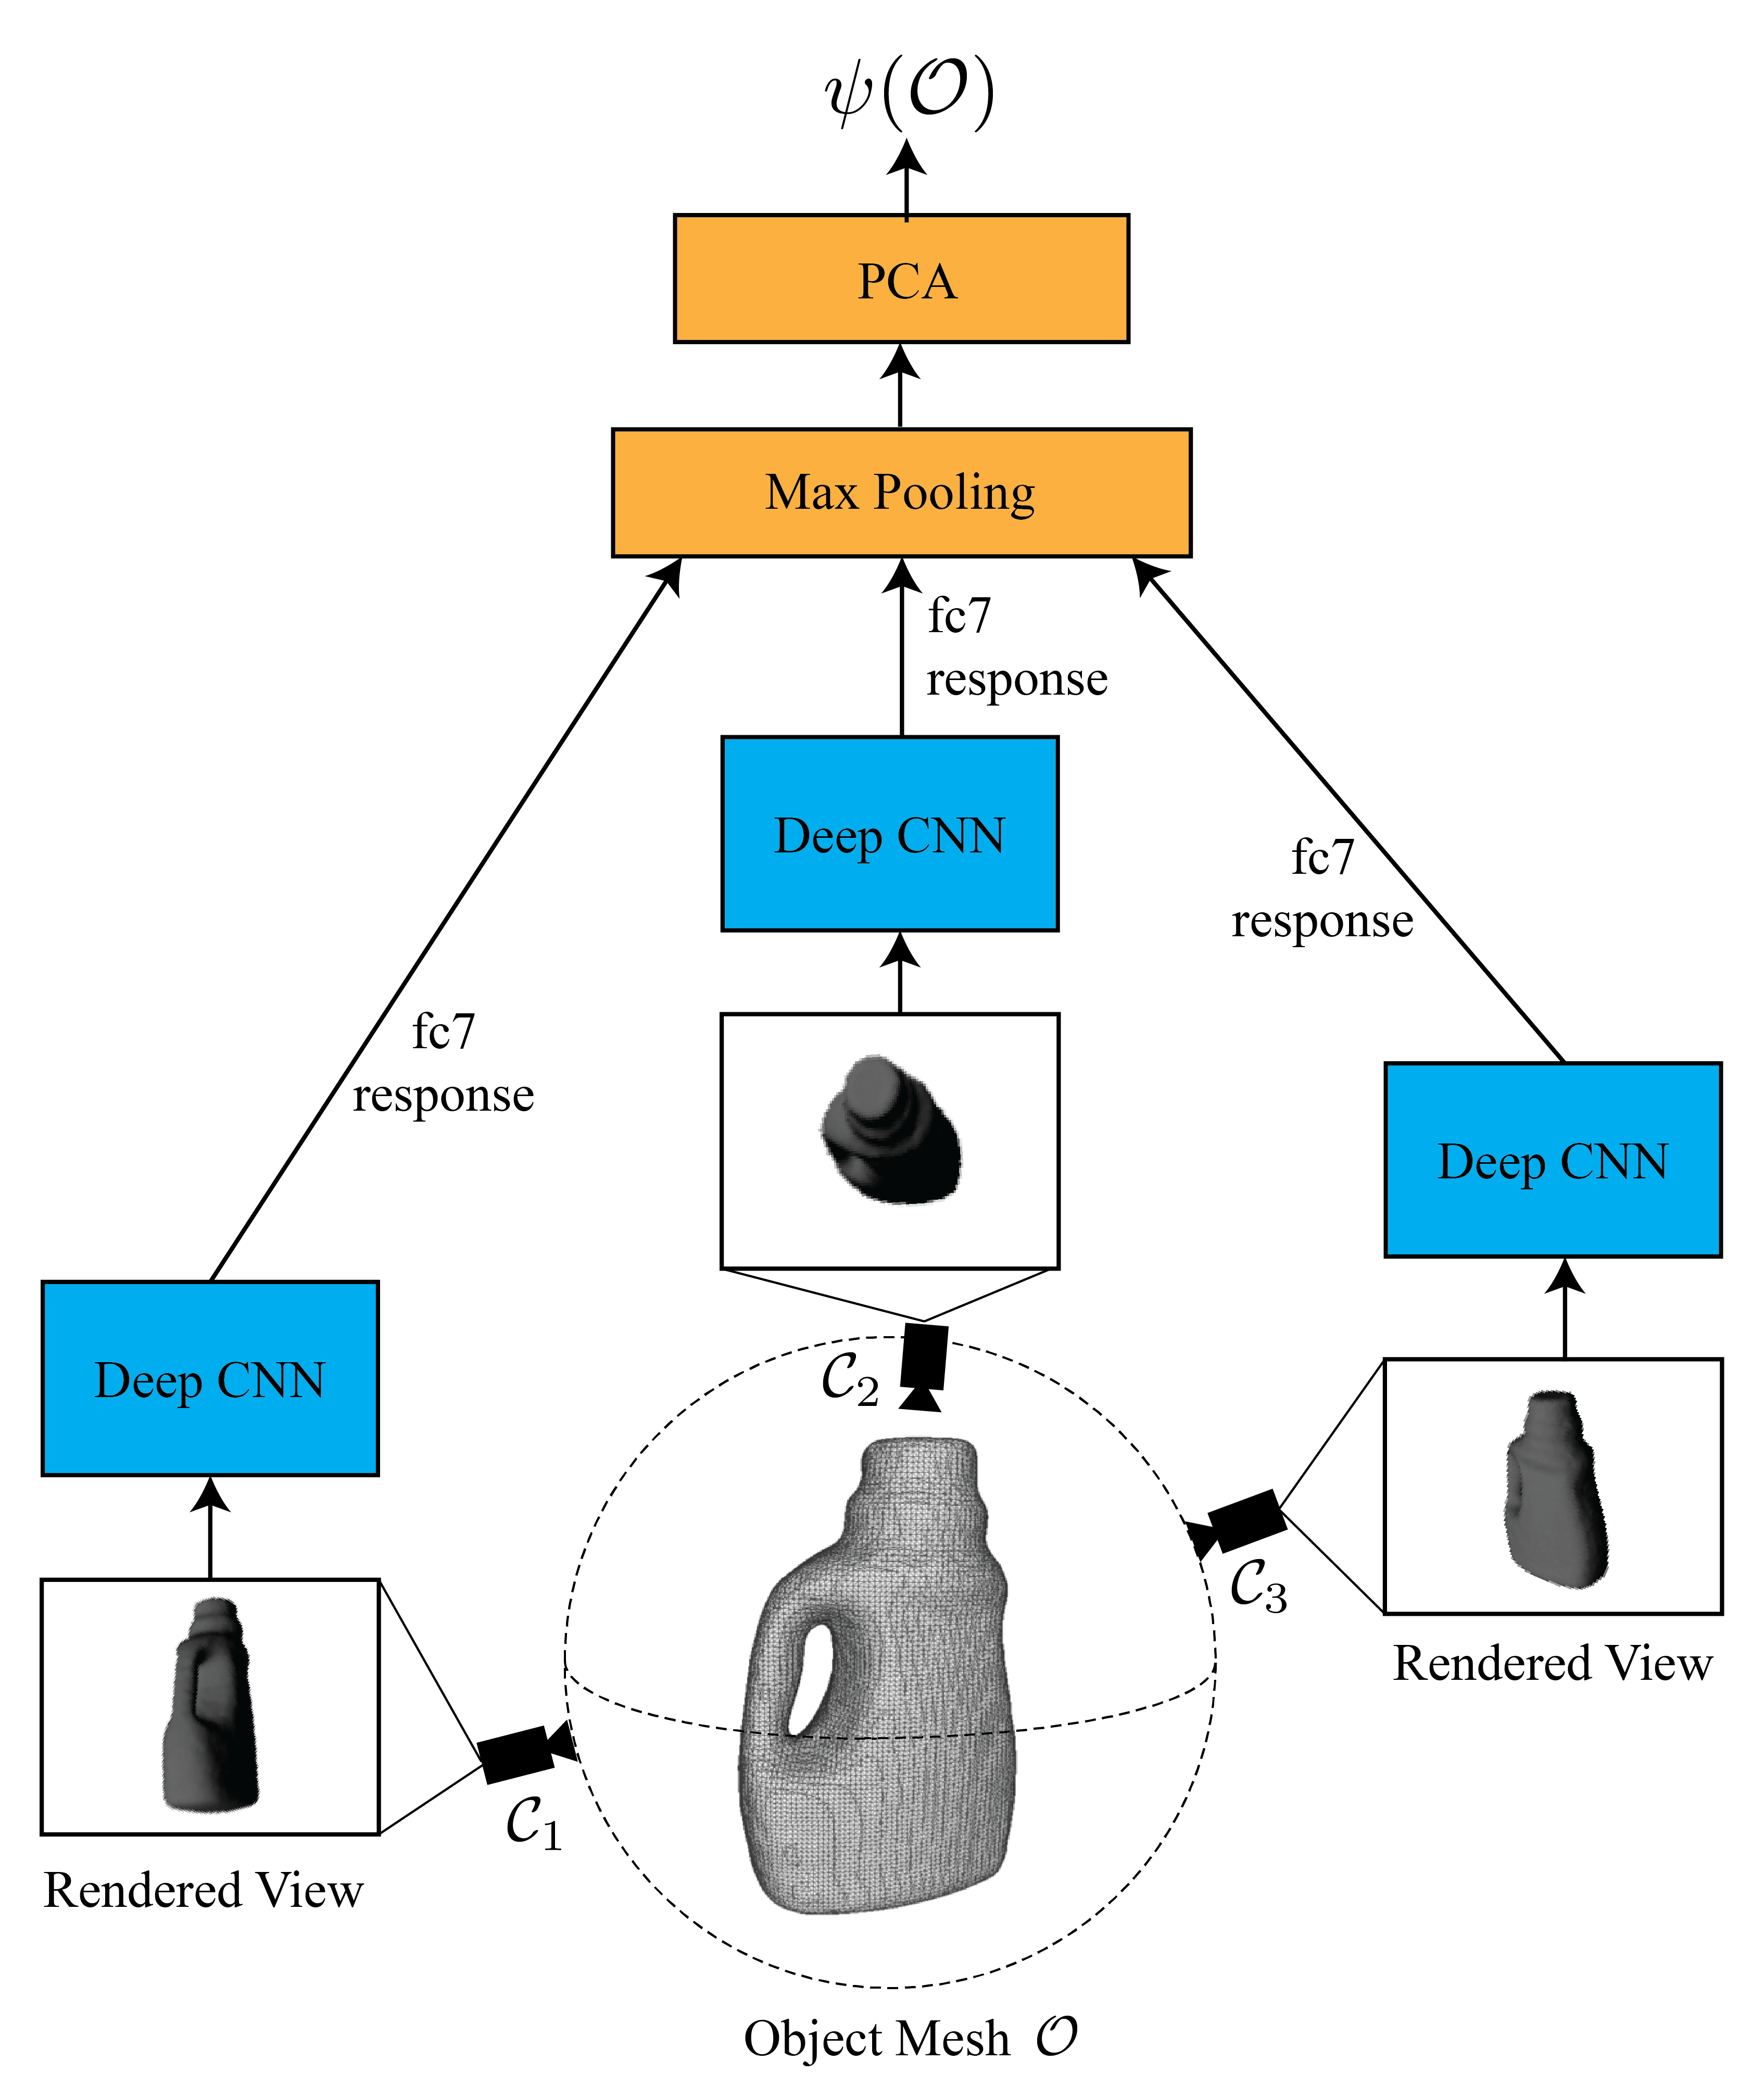
\includegraphics[scale=0.3]{figures/illustrations/cnn_model.png}
\caption{Illustration of our method for embedding 3D object models in a Euclidean vector space for computing global shape similiarty. We pass a set of 50 virtually rendered camera viewpoints discretized around a sphere through a deep Convolutional Neural Network (CNN) with the AlexNet~\cite{krizhevsky2012imagenet} architecture. Finally, we take the maximum fc7 response across each of the 50 views for each dimension and run PCA to reduce the dimensionality of the output.}
\figlabel{global-feature-model}
\vspace*{-15pt}
\end{figure}

\subsection{Optimizing Feature Weights}
One remaining issue is the selection of the relative feature weights $w_1, ..., w_{N_f}$.
Past work has optimized these weights using a squared error loss on the probability of success predicted by the CCBP and a true probability of success from brute force evaluation~\cite{montesano2012active}.
However, this criterion may be inappropriate for predicting probabilities, as the predictions must be bounded between 0 and 1.
In this work we instead select the weights which minimze the cross entropy loss~\cite{}:

\begin{align*}
	w_1^*, ..., w_{N_f}^* = \myargmin{w_1 \geq 0, ..., w_{N_f} \geq 0} \frac{1}{M} \sum \limits_{i=1}^M &\mu_i \log \left( \frac{\alpha_i}{\alpha_i + \beta_i} \right) + \\  &(1 - \mu_i) \log \left( \frac{\beta_i}{\alpha_i + \beta_i} \right)
\end{align*}
\noindent where $\alpha_i$ and $\beta_i$ are the posterior shape parameters given by Equations~\ref{eq:alpha} and~\ref{eq:beta} and $\mu_i$ is the known probability of force closure evaluated by exhaustive Monte-Carlo integration for a set of $M$ grasps.
We optimize this objective using Stochastic Gradient Descent (SGD) with the weights all initialized to 100.
%\input{includes/methodology}
%\input{includes/analysis}
%\section{Experiments}
\seclabel{experiments}

We evaluate the convergence rate of the Dex-Net 1.0 algorithm for varying sizes of prior data used from Dex-Net and explore the sensitivity of the convergence rate to object shape, the similarity kernel bandwidths, and uncertainty.
We created two training sets of 1000, and 10000 objects by uniformly sampling objects from Dex-Net.
We uniformly sampled a set of 300 validation objects for selecting algorithm hyperparameters and selected a set of 45 test objects from the remaining objects.
We ran the algorithm with $N_n = 10$ nearest neighbors, $\alpha_0 = \beta_0 = 1.0$~\cite{laskey2015bandits}, and a lower confidence bound for 75\% of the belief distribution.
We used isotropic Gaussian uncertainty with object and gripper translation variance $\sigma_{t} = 0.005$, object and gripper rotation variance $\sigma_{r} = 0.1$, and friction variance $\sigma_{\gamma} = 0.1$.

The inverse bandwidths of the similarity kernel were $C_g = diag(0,0,175, 175)$ for the grasp parameter features, an isotropic Gaussian mask $C_d$ with mean $\mu_d = 500.0$ and $\sigma = 1.75$ for the differential heightmap features, and $C_s = 0.001 I$ for the shape similarity features.
The bandwidths were selected by maximizing the log-likelihood of the true $P_F$ under the CCBP model~\cite{goetschalckx2011continuous} on the validation set using a grid search over hyperparameters.

To scale the experiments, we developed a Cloud-based system on top of Google Cloud Platform.
We used Google Compute Engine (GCE) to distribute trials of MAB algorithms across objects and Google Cloud Storage to store Dex-Net.
The system launched up to 1500 GCE single core instances each with 3.75 GB of memory at once for hyperparameter tuning and convergence analysis, reducing the runtime of experiments by over 1000$\times$.

\subsection{Scaling of Average Convergence Rate}
\seclabel{conv-rate}
To examine the effects of orders of magnitude of prior data on convergence to a grasp with high $P_F$, we ran the Dex-Net 1.0 algorithm on the test objects with priors computed from 1,000 and 10,000 objects from Dex-Net. 
~\figref{avg-reward} shows the normalized $P_F$ versus iteration averaged over 25 trials for each of the test objects for 2,000 iterations.
The plot compares the Dex-Net algorithm to Thompson sampling without priors (TS) and uniform allocation (UA)~\cite{laskey2015bandits}.
The algorithm with 10,000 objects takes approximately $3.5\times$ fewer iterations to reach the maximum normalized $P_F$ value reached by TS.
Furthermore, the 10,000 object curve does not fall below 90\% of the best grasp in the set across all iterations, suggesting that a grasp with high $P_F$ is found using prior data alone.

\begin{figure}[t!]
\centering
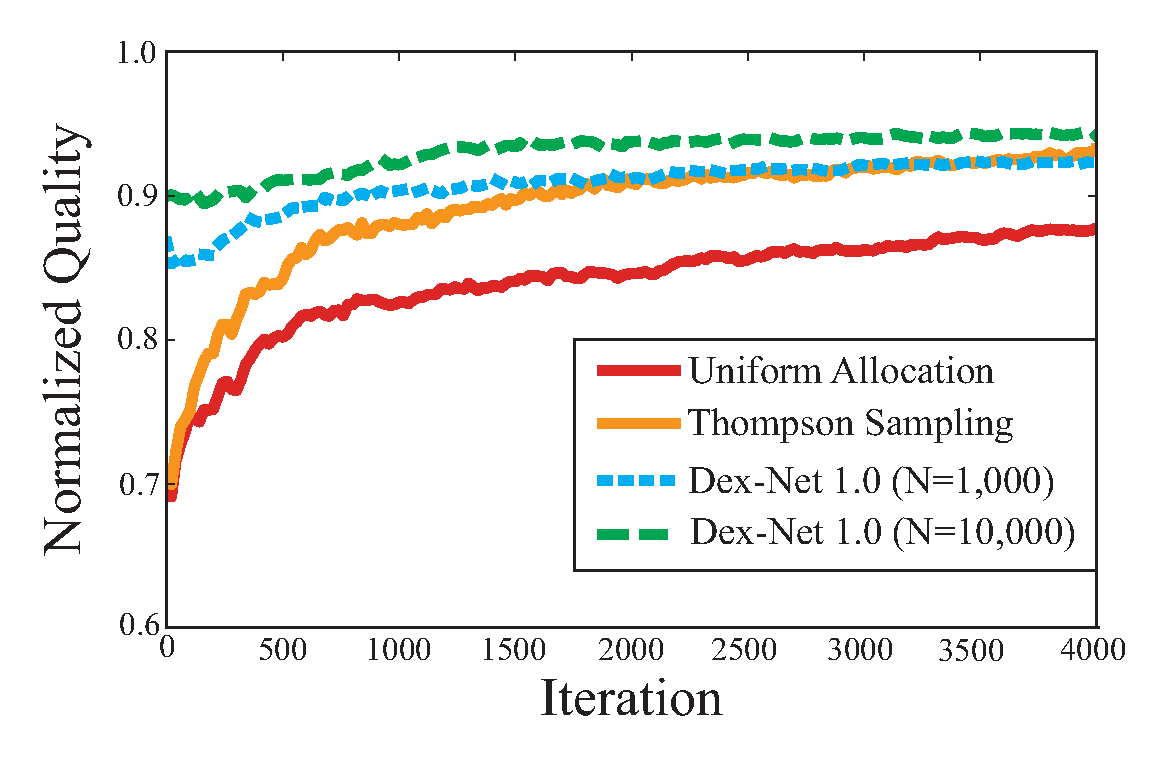
\includegraphics[scale=0.40]{figures/illustrations/avg_reward.eps}
\caption{Average normalized grasp quality versus iteration over 45 test objects and 25 trials per object for the Dex-Net algorithm with 1,000 and 10,000 prior 3D objects from Dex-Net. We measure quality by the $P_F$ for the best grasp predicted by the algorithm on each iteration and compare with Thompson sampling without priors and uniform allocation. The algorithm converges faster with 10,000 models, never dropping below approximately 90\% of the grasp with highest $P_F$ from the 250 candidate set.}
\figlabel{avg-reward}
\vspace*{-10pt}
\end{figure}

\subsection{Sensitivity to Object Shape}
\seclabel{shape-sens}
To understand the behavior of the Dex-Net algorithm on individual 3D objects, we examined the convergence rate with a 3D model of a drill and spray bottle from the test set, both uncommon object categories in Dex-Net.
\figref{avg-reward-spray} and  \figref{avg-reward-drill} show the normalized $P_F$ (the ratio of the $P_F$ for the sampled grasp to the highest $P_F$ of the 250 candidate grasps) versus iteration averaged over 25 trials for 2,000 iterations on the spray bottle and drill, respectively.
We see that the spray bottle converges very quickly when using a prior dataset of 10,000 objects, finding the optimal grasp in the set in about 1,500 iterations.
This convergence may be explained by the two similar spray bottles retrieved by the MV-CNN from the 10,000 object dataset.
\figref{spray-grasps} illustrates the grasps predicted to have the highest $P_F$ on the spray bottle by the different algorithms after 100 iterations.
However, performance on the drill does not increase using either 1,000 or 10,000 objects, as the closest model in all of Dex-Net according to the similarity metric is a phone.

\begin{figure}[t!]
\centering
\includegraphics[scale=0.41]{figures/illustrations/drill_avg_reward_w_neighbors.eps}
\caption{Average normalized grasp quality versus iteration over 25 trials for the Dex-Net 10 algorithm with 1,000 and 10,000 prior 3D objects (bottom) and illustrations of five nearest neighbors in Dex-Net (top) for a drill. (Top) The drill, which is relatively rare in the dataset, has no geometrically similar neighbors even with 10,000 objects. (Bottom) This leads to no significant performance increase over Thompson sampling.}
\figlabel{avg-reward-drill}
\vspace*{-10pt}
\end{figure}

\begin{figure}[t!]
\centering
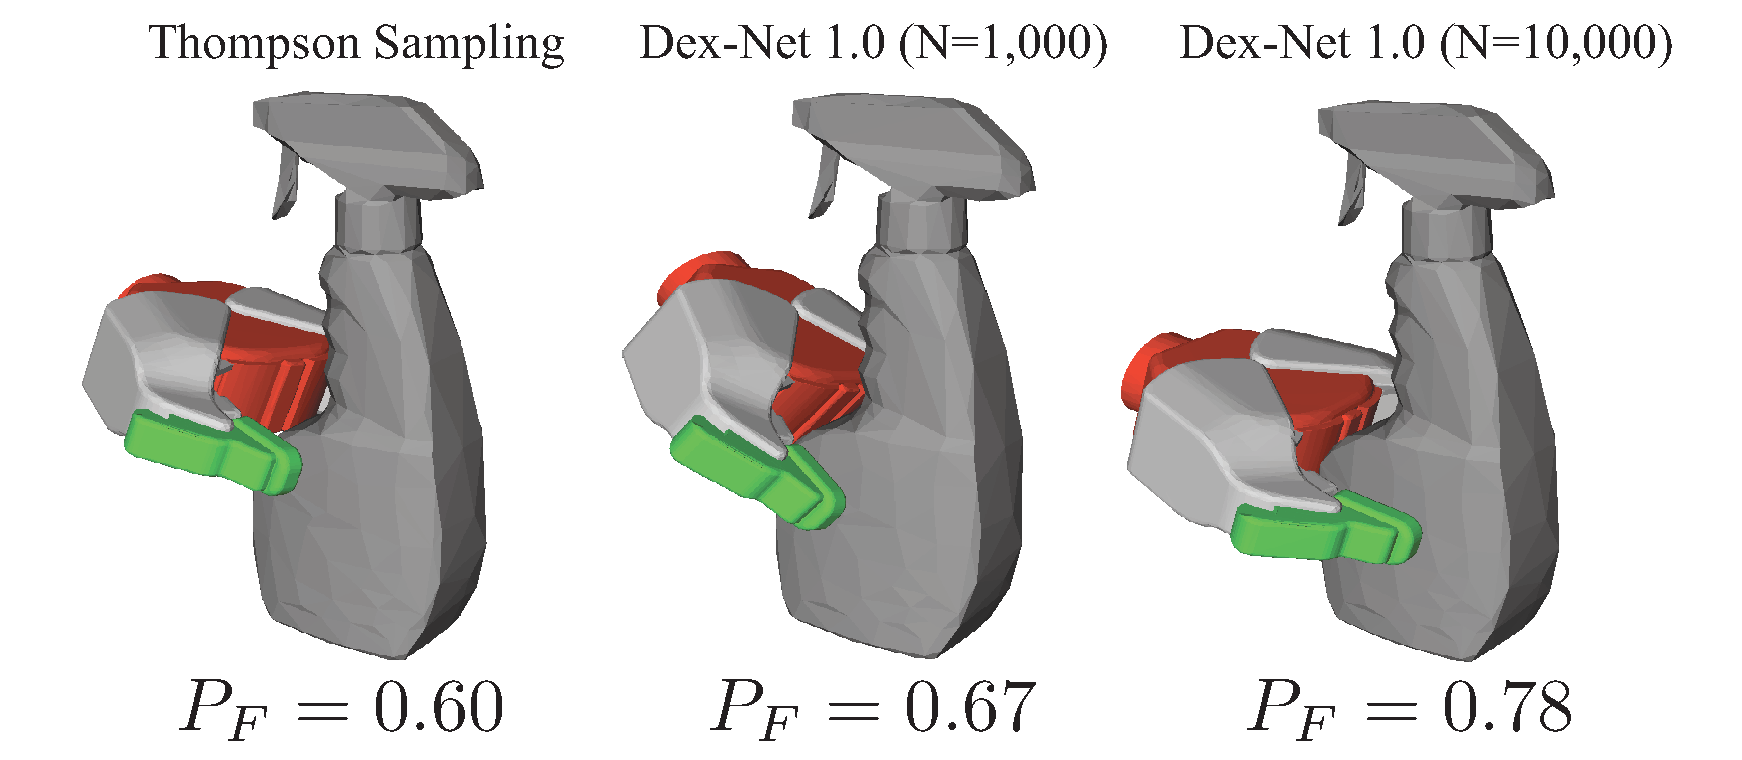
\includegraphics[scale=0.28]{figures/illustrations/spray_grasps.eps}
\caption{Illustation of the grasps predicted to have the highest $P_F$ after only 100 iterations by Thompson sampling without priors and the Dex-Net algorithm with 1,000 and 10,000 prior objects. Thompson sampling chooses a grasp near the edge of the object, while the Dex-Net algorithm selects grasps closer to the center-of-mass of the object.}
\figlabel{spray-grasps}
\vspace*{-5pt}
\end{figure}

\subsection{Sensitivity to Similarity and Uncertainty}
\seclabel{band-sens}
We also studied the sensitivity of the Dex-Net algorithm to the kernel bandwidth hyperparameters described in \secref{ccbps} and the levels of pose an friction uncertainty for the test object.
We varied the inverse bandwidths of the kernel for the grasp parameters and differential heightmaps gradients to the lower values $C_g = diag(0,0,15, 15)$, $\mu_d = 350.0$,  and $\sigma = 3.0$ as well as the higher values $C_g = diag(0,0,300, 300)$, $\mu_d = 750.0$,  and $\sigma = 1.75$.
We also tested low uncertainty with object and gripper translation variance $\sigma_{t} = 0.0025$, object and gripper rotation variance $\sigma_{r} = 0.05$, and friction variance $\sigma_{\gamma} = 0.05$ as well as high uncertainty: $\sigma_{t} = 0.01, \sigma_{r} = 0.2,$ and $\sigma_{\gamma} = 0.2$.
\figref{bnu-sens} shows the normalized $P_F$ versus iteration averaged over 25 trials for 2,000 iterations on the 45 test objects.
The results suggest that conservative setting of similiarity kernel bandwidth is important for convergence and that the algorithm is not sensitive to uncertainty levels.

\begin{figure}[t!]
\centering
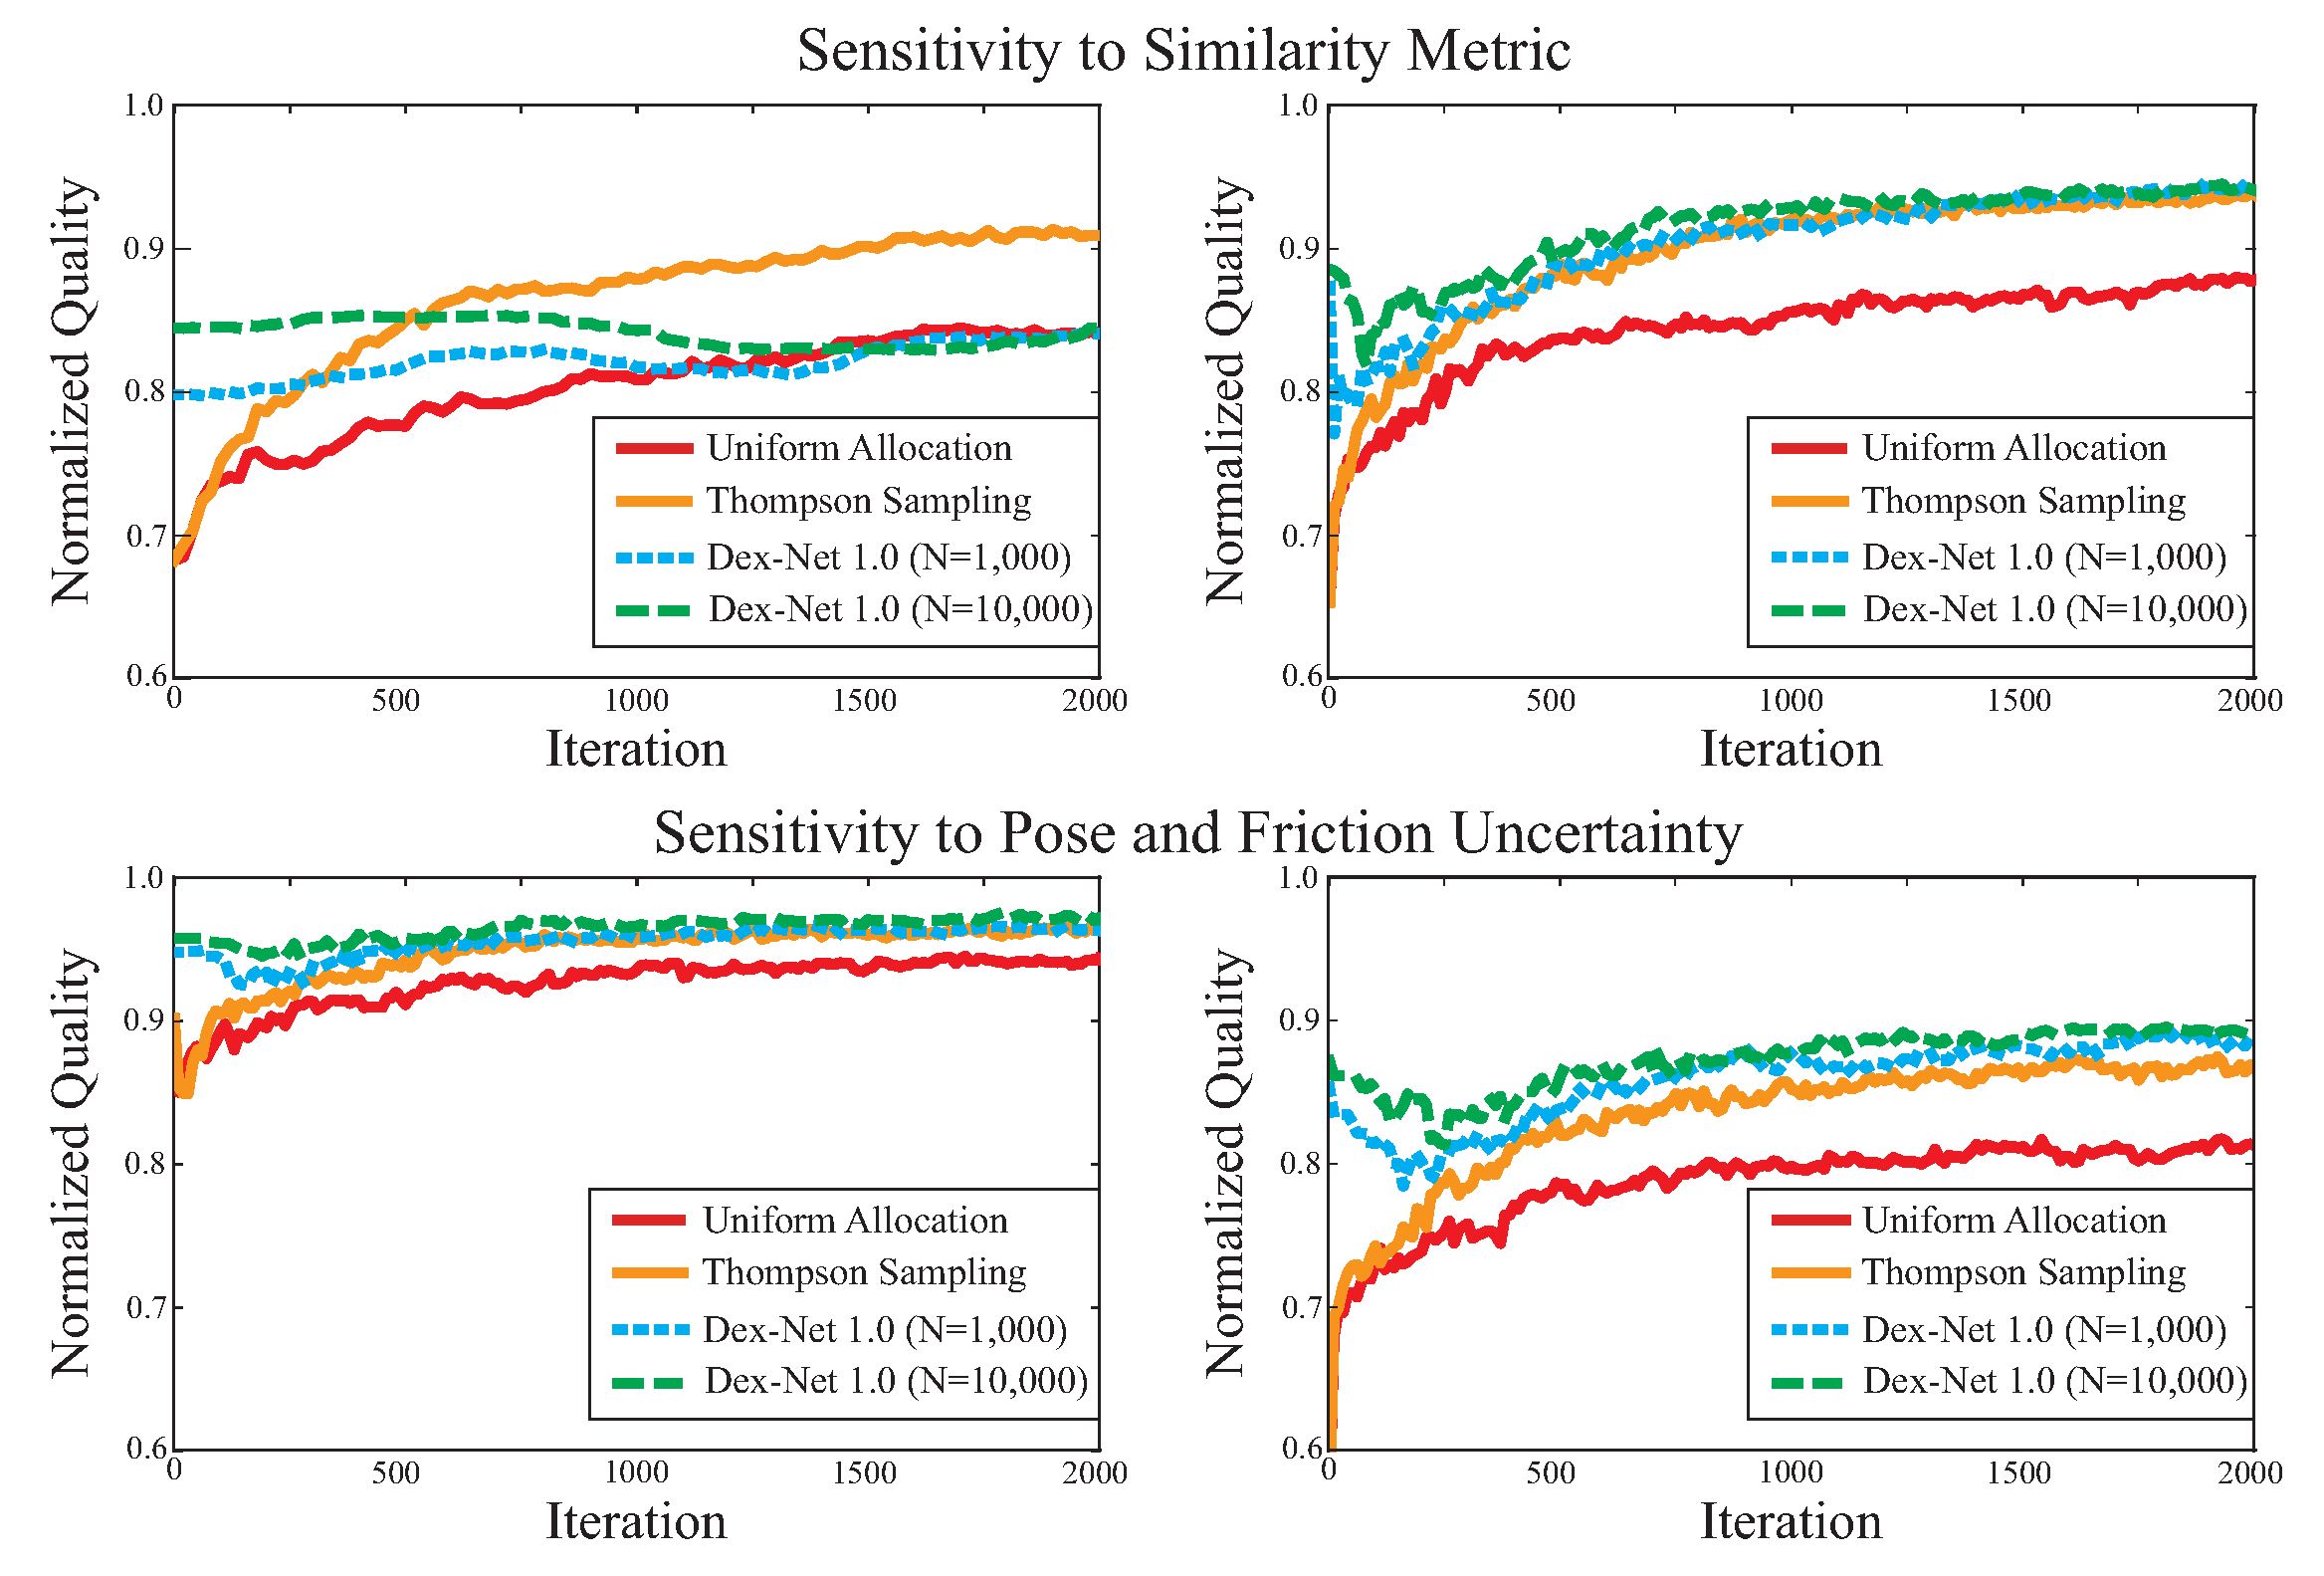
\includegraphics[scale=0.22]{figures/illustrations/combined_weight_and_u_sensitivity.eps}
\caption{Sensitivity to similiarity kernel (top) and pose and friction uncertainty (bottom) for the average normalized grasp quality versus iteration over 25 trials per object for the Dex-Net algorithm with 1,000 and 10,000 prior 3D objects.
%with a higher heightmap gradient kernel bandwidth of $1 / 350$ (left) and a lower kernel bandwidth of $1 / 450$ (right).
(Top-left) Using a higher inverse bandwidth causes the algorithm to measure false similarities between grasps, leading to performance on par with uniform allocation.
(Top-right) A lower inverse bandwith decreases the convergence rate, but on average the Dex-Net Algorithm still selects a grasp within approximately 85\% of the grasp with highest $P_F$ for all iterations.
(Bottom-left) Lower uncertainty increases the quality for all methods and (bottom-right) higher uncertainty decreases the quality for all methods, and the Dex-Net algorithm with 10,000 prior objects still converges approximately 2$\times$ faster than Thompson sampling without priors. 
}
\figlabel{bnu-sens}
\vspace*{-15pt}
\end{figure}
%\section{Discussion and Future Work}
\seclabel{conclusion}
We presented Dexterity Network 1.0 (Dex-Net), a new dataset and associated algorithm to study the scaling effects of Big Data and Cloud Computation on robust grasp planning.
The algorithm uses a Multi-Armed Bandit model with correlated rewards to leverage prior grasps and 3D object models and Multi-View Convolutional Neural Networks (MV-CNNs), a new deep learning method for 3D object classification, as a similarity metric between objects.
In experiments, the Google Cloud Platform allowed Dex-Net 1.0 to simultaneously run up to 1,500 virtual machines, reducing experiment runtime by three orders of magnitude.
Experiments suggest that prior data can speed robust grasp planning by a factor of 2 and that average grasp quality increases with the number of similar objects in the dataset.
We reported on sensitivity to varying similarity metrics and pose and friction uncertainty levels.

In future work, we will develop metrics to pre-compute grasps that adequately ``cover" each object from a variety of accessibility conditions (depending on pose and occlusions).
We will also explore how Deep Learning~\cite{krizhevsky2012imagenet} can be used in other parts of a grasp planning pipeline, for example to recognize object pose and shape from images~\cite{aubry2015understanding}, to learn grasp and object features robust to shape variation using prior evaluations from bandit algorithms, and perhaps even to determine motor torques based on images and precomputed grasps~\cite{levine2015end}.
We also hope to release subsets of Dex-Net 1.0 with an open-source API to explore robust grasping as a service (RGaaS).



%%\appendix
%\include{includes/proofs}

\addtolength{\textheight}{-9.0cm}

%\balance
\bibliographystyle{IEEEtranS}
\bibliography{bibliography}



\end{document}



